\chapter{HeROfake : Orchestration serverless sur ressources hétérogènes pour le cloud privé}

\section{Introduction}
\label{section:herofake-introduction}

\begin{table*}[t]
    \centering
    \caption{State of the Art work on autoscaling platforms}
    \resizebox{\textwidth}{!}{
        \begin{tabular}{lccccccc}
            \toprule
            & Serverless & Target cloud platform     & SLA & Hardware heterogeneity & Resources usage & Energy consumption & Cost-aware \\
            \cmidrule(lr){2-2}\cmidrule(lr){3-3}\cmidrule(lr){4-4}\cmidrule(lr){5-5}\cmidrule(lr){6-6}\cmidrule(lr){7-7}\cmidrule(lr){8-8}
            Swayam~\cite{gujaratiSwayamDistributedAutoscaling2017}        & \xmark         & Private (Azure, in-house) & \cmark& \xmark                     & \cmark            & \xmark                 & \xmark         \\
            Pigeon~\cite{lingPigeonDynamicEfficient2019}                  & \cmark       & Private                   & \xmark  & \cmark                   & \cmark            & \xmark                 & \xmark         \\
            MArk~\cite{zhangMArkExploitingCloud}                          & \xmark         & Public (AWS)              & \cmark& \cmark                   & \cmark            & \xmark                 & \cmark       \\
            ENSURE~\cite{sureshENSUREEfficientScheduling2020}             & \cmark       & Private                   & \xmark  & \xmark                     & \cmark            & \xmark                 & \cmark       \\
            Mampage et al.~\cite{mampageDeadlineawareDynamicResource2021} & \cmark       & Private                   & \cmark& \xmark                     & \cmark            & \xmark                 & \cmark       \\
            Atoll~\cite{singhviAtollScalableLowLatency2021}               & \cmark       & Private                   & \cmark& \xmark                     & \xmark              & \xmark                 & \xmark         \\
            INFless~\cite{yangINFlessNativeServerless2022}                & \cmark       & Private                   & \cmark& \xmark                     & \cmark            & \xmark                 & \cmark       \\
            SMIF~\cite{choSLADrivenMLInference}                           & \cmark       & Private                   & \cmark& \cmark                   & \cmark            & \xmark                 & \xmark         \\
            Target solution                                                & \cmark       & Private                   & \cmark& \cmark                   & \cmark            & \cmark               & \cmark       \\ \bottomrule
        \end{tabular}
    }
    \label{table:herofake-sota}
\end{table*}

\textbf{Modèle serverless}. Le serverless peut être compris à la fois comme un modèle de programmation, appelé Function as a Service (FaaS), et comme un modèle de déploiement pour le cloud. Dans un tel modèle, les développeurs conçoivent leurs applications comme une composition de fonctions sans état dont l'exécution est pilotée par des événements~\cite{SchleierSmith2021WhatSC}. 
Les services serverless libèrent les locataires d'une réservation complexe des ressources, car ils sont conçus pour gérer les exigences de mise à l'échelle à la demande.

Dans le modèle FaaS, les fournisseurs ne facturent les clients qu'en fonction de leur utilisation réelle des ressources~\cite{jonasCloudProgrammingSimplified2019}. Ils sont entièrement responsables du déploiement d'une gestion intelligente des ressources et du multiplexage à une granularité plus fine afin d'optimiser les mesures de qualité de service (QoS) telles que le temps de réponse, la consommation d'énergie, etc.

\textbf{Détection de deepfake et serverless}. Le travail présenté dans cet article faisait partie d'un projet (à l'institut de recherche b{\textless\textgreater}com \footnote{\href{https://b-com.com/en}{https://b-com.com/en}}) visant à déployer un service de détection de deepfake économe en énergie dans un cloud hétérogène. Les deepfakes sont des images, des vidéos ou des discours synthétiques, créés numériquement pour imiter une personne existante de manière à tromper les spectateurs. La détection de deepfake consiste à entraîner un réseau neuronal convolutif (CNN) pour détecter des modèles d'incohérences introduits dans le processus de création.

Les fonctions utilisées par notre application deepfake répondent à trois caractéristiques principales pour des charges de travail serverless adaptées~\cite{cncf2018whitepaper} : leur exécution peut être rendue parallèle (plusieurs images indépendantes), elles sont stateless (pure transformation sur les données d'entrée) et event-driven (lancées après l'upload des données).

D'une part, la détection de deepfake à l'aide de réseaux de neurones convolutifs (CNN) est une tâche qui peut tirer parti de la concurrence en exécutant plusieurs convolutions en parallèle et/ou en traitant différentes images sur plusieurs threads. Ces tâches sont essentiellement sans état, car elles appliquent une transformation pure sur les données d'entrée - en prenant une image en entrée et en renvoyant une valeur booléenne en sortie. Une telle application est pilotée par les événements, le calcul commençant après le téléchargement d'une image d'entrée. Ce sont là trois caractéristiques principales des charges de travail serverless appropriées~\cite{cncf2018whitepaper}.

D'autre part, les ressources matérielles nécessaires pour exécuter cette application à l'échelle seraient nombreuses et coûteuses : être en mesure de faire évoluer dynamiquement les ressources en fonction de la demande permettrait au client de réaliser d'importantes économies et au fournisseur d'accepter plus de clients sur le même nombre de nœuds.

Par conséquent, nous soutenons que le modèle de service serverless est parfaitement adapté à l'inférence à la demande rentable utilisant des CNN.

\textbf{Hétérogénéité matérielle dans le cloud}. Les infrastructures cloud sont de plus en plus hétérogènes pour répondre aux besoins des applications à forte intensité de données telles que l'apprentissage automatique de modèles ou l'analyse de données massives~\cite{reissHeterogeneityDynamicityClouds}. Cependant, les processeurs spécialisés et les GPU doivent encore être mis à la disposition des clients dans les offres serverless~\cite{khandelwalTaureauDeconstructingServerless2020}. L'accélération matérielle devrait être décidée par le fournisseur sur la base d'une application ou d'une demande.

Les travaux de l'état de l'art montrent que l'utilisation de ce matériel dans un cadre cloud permet des gains substantiels en termes de temps d'exécution et de consommation d'énergie~\cite{10.1145/3369583.3392679, 9195730}. Cependant, les orchestrateurs de référence tels que Kubernetes avec Knative ou OpenWhisk ne prennent pas en charge l'allocation dynamique de ce type de matériel.

\textbf{Défi de performance pour le déploiement serverless}. En raison de la nature transitoire des ressources FaaS non réservées, la latence, le débit et la continuité du service sont difficiles à garantir~\cite{vaneykSPECRGCloud2018, dartoisCuckooOpportunisticMapReduce2019}. Lorsque les applications ne reçoivent pas de demandes entrantes, les bacs à sable des fonctions sont détruits au lieu d'être maintenus dans un état d'inactivité. Ensuite, lorsqu'une nouvelle demande arrive, le fournisseur doit (ré)allouer des ressources et initialiser des fonctions pour déployer de nouveaux bacs à sable : c'est ce qu'on appelle un démarrage à froid. Les temps de démarrage à froid sont très pénalisants pour les performances de l'application, ils peuvent même dominer les temps d'exécution totaux~\cite{mullerLambadaInteractiveData2020}.

De plus, dans les offres commerciales serverless actuelles, les accords de niveau de service (SLA) sont généralement limités à des tentatives automatisées (redémarrages) en cas d'échec, et les fournisseurs de FaaS limitent généralement le temps d'exécution des fonctions serverless à quelques minutes. L'absence de garanties de qualité de service dans les offres commerciales serverless les empêche d'être plus largement utilisées~\cite{buyyaSLAorientedResourceProvisioning2011}.

\textbf{Énoncé du problème -- mettre tout ensemble}. Le problème que nous tentons de résoudre dans cet article est de déterminer comment dimensionner automatiquement et de manière réactive des ressources matérielles hétérogènes dans le cloud en fonction de la charge sur l'application et des exigences de qualité de service des utilisateurs, tout en maintenant le coût des ressources et de l'énergie au niveau le plus bas possible pour le fournisseur. Nous considérons une application de détection de deepfake comme cas d'étude pour² notre travail.

\textbf{État de l'art}. Des études antérieures ont exploré le besoin d'une plateforme de mise à l'échelle automatique qui prend en charge les tâches de courte durée comprises dans des applications telles que l'apprentissage automatique en tant que service. Le tableau~\ref{table:herofake-sota} résume les différences entre ces solutions et la plateforme cible que nous essayons d'atteindre, et la section~\ref{section:herofake-sota} fournit des détails supplémentaires. Bien que de nombreuses études aient établi la nécessité d'une accélération à la demande comme solution pour garantir le temps de réponse des fonctions, aucune n'a mesuré l'impact de l'exploitation des ressources hétérogènes sur la consommation d'énergie dynamique. En outre, les études précédentes considèrent la consolidation des tâches comme un moyen de libérer des ressources pour d'autres calculs - nous soutenons que ces techniques ouvrent des possibilités pour le fournisseur de services d'appliquer des politiques d'économie d'énergie dans le cloud privé. Enfin, comme les plateformes serverless sont à usage général et conçues pour être hautement configurables, notre solution cible devrait être consciente des coûts pour permettre au fournisseur de faire des choix de configuration se rapportant à leurs propres objectifs.

\textbf{Notre contribution}. Nous soutenons que l'utilisation opportuniste des accélérateurs matériels (GPU et FPGA) pour planifier les tâches de détection de deepfake peut permettre aux fournisseurs de cloud de garantir le temps de réponse des tâches serverless et d'atteindre le SLA tout en réduisant l'utilisation des ressources et la consommation d'énergie.

Dans cet article, nous proposons un cadre complet pour déployer une application de détection de deepfake sur un cloud serverless. Ce cadre comprend une phase hors-ligne et une phase en ligne. Le \textbf{phase hors-ligne} est utilisé pour caractériser la performance et le comportement énergétique des plates-formes matérielles hétérogènes déployées. La \textbf{phase en ligne} consiste en une plateforme de mise à l'échelle automatique et une stratégie d'ordonnancement qui utilisent efficacement les ressources matérielles hétérogènes (caractérisées) pour atteindre les accords de niveau de service par demande tout en réduisant la consommation d'énergie de la plateforme. 

Pour cette étude de cas, nous avons conçu un environnement de simulation qui modélise l'infrastructure d'une application de détection de deepfake, exécutée par le fournisseur en tant que Software as a Service à l'aide d'une infrastructure serverless.

\textbf{Certains chiffres de performance}. Avec notre politique d'allocation et d'ordonnancement, nous avons été en mesure de traiter 50000 tâches dans le même makespan que Knative avec moins de 36\% de pénalités de QoS. Notre cadre réduit la consommation d'énergie pour l'exécution des tâches de près de 35\% et permet au fournisseur de réduire davantage la consommation d'énergie statique en consolidant les tâches sur moins de 29\% des nœuds disponibles.

Le document est organisé comme suit : dans une première section, nous décrivons le modèle de plateforme global pour le projet. Ensuite, nous décrivons la plateforme d'exécution et la phase de caractérisation de la charge de travail. Dans la section III, nous décrivons les défis de l'orchestration de ressources serverless, notre modèle de tâches et les politiques d'allocation et d'ordonnancement de l'orchestrateur. La section IV présente notre méthodologie d'évaluation et une discussion des résultats expérimentaux. La section V donne des détails concernant l'état de l'art sur les plateformes d'autoscaling. Enfin, nous concluons par quelques perspectives pour les travaux futurs.

\section{Déployer des tâches de détection de deepfake dans un cloud serverless}
\label{section:herofake-deepfake}

\begin{figure*}[t]
\centering
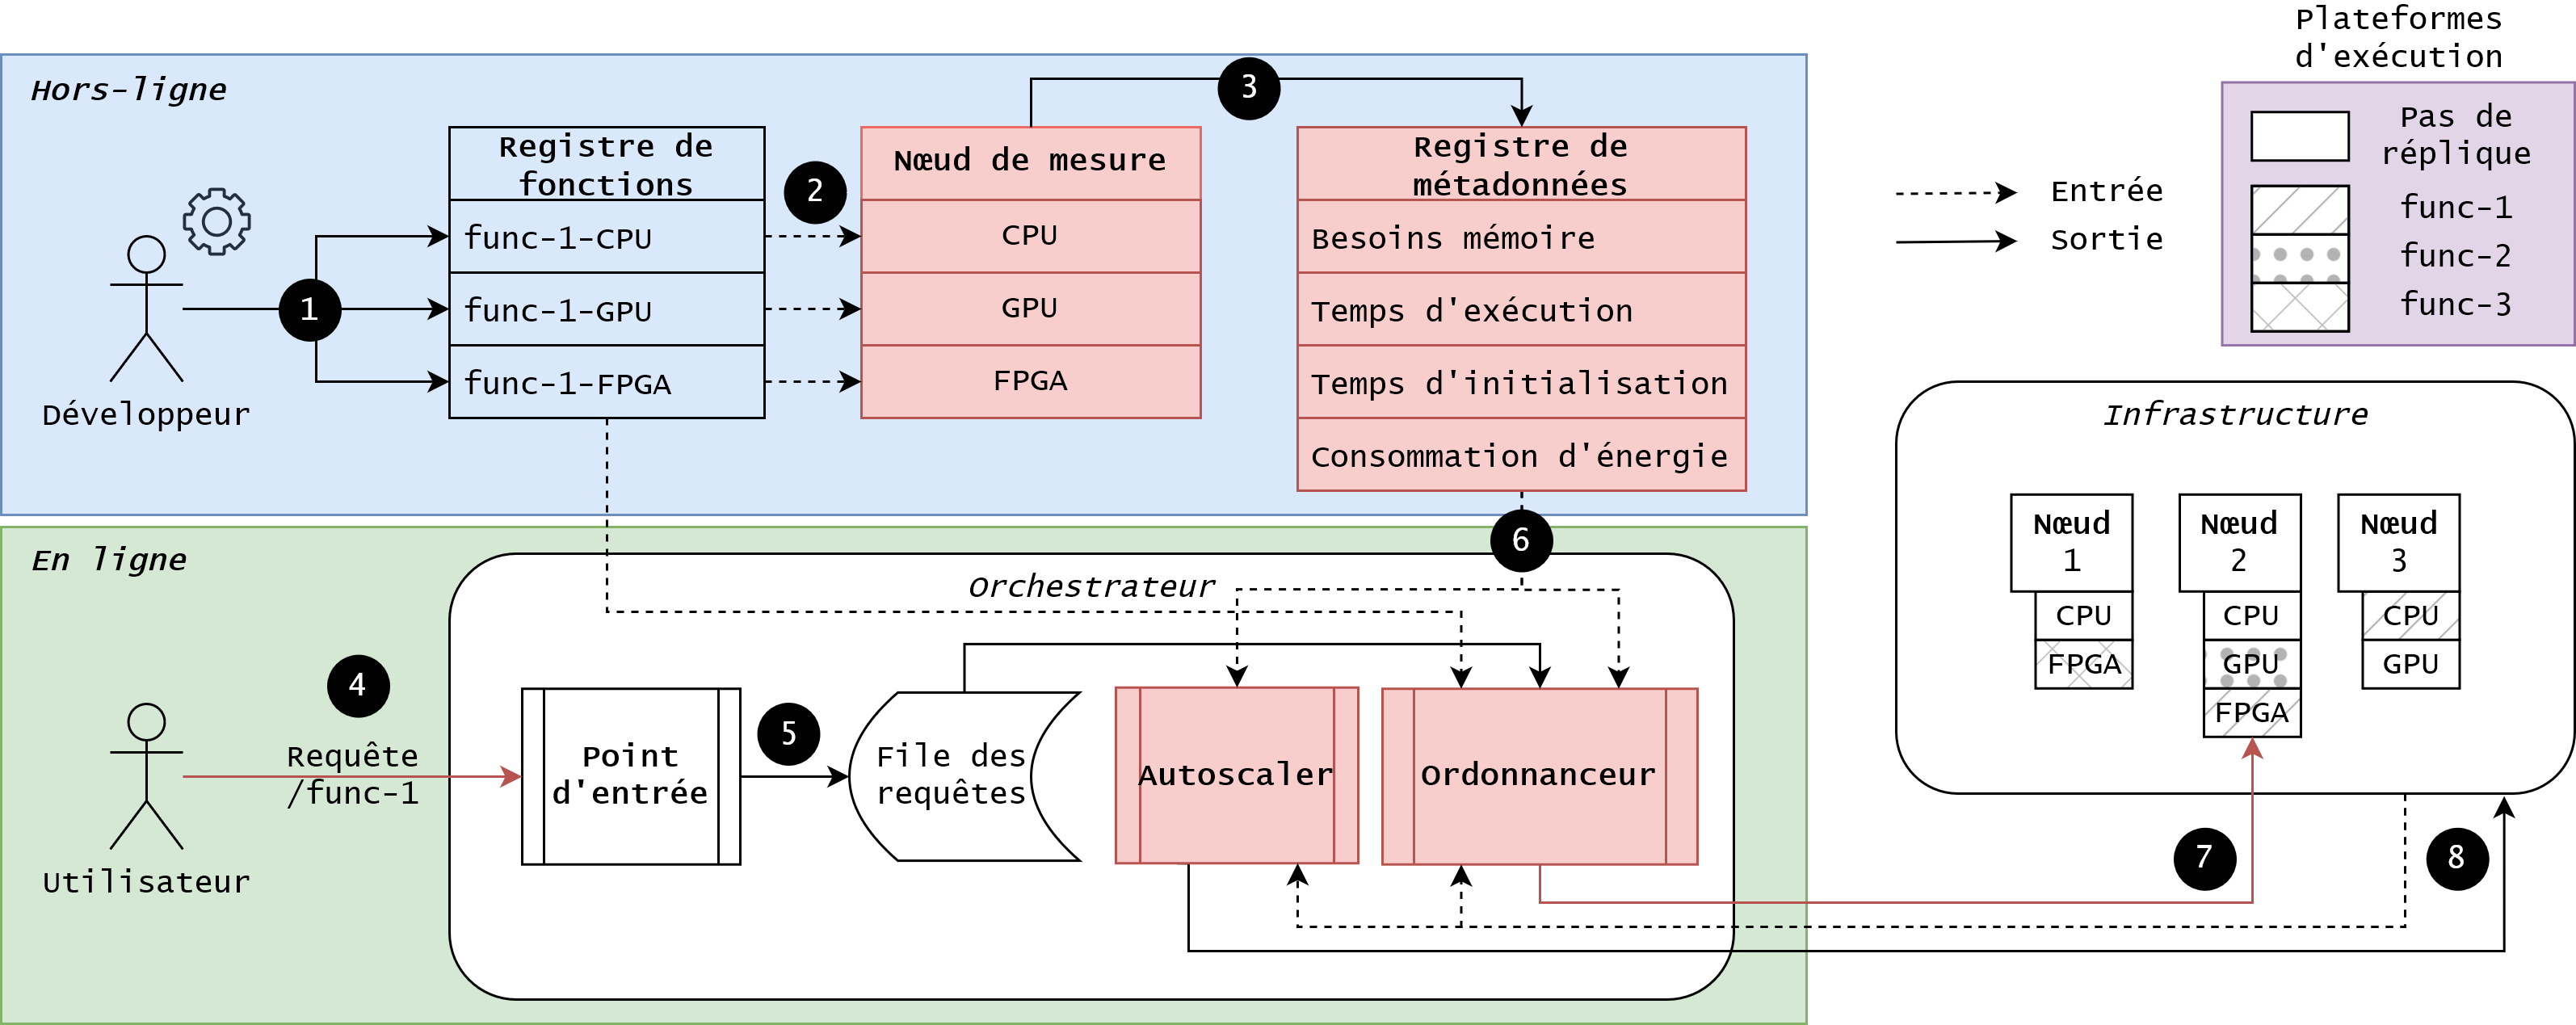
\includegraphics[width=0.8\textwidth]{4_Chapitre4/figures/placement.png}
\caption{Plateforme de détection de deepfake serverless, vue d'ensemble du système.}
\label{figure:herofake-placement}
\end{figure*}

Cette section présente le modèle de plateforme serverless utilisé et le projet global.

\subsection{Modèle de la plateforme}

Nous considérons un système de détection de deepfake qui est déployé comme une application serverless composée de trois fonctions sans état qui réalisent des tâches d'inférence sur des images d'entrée. Ces images sont toutes RVB et de taille $224 * 224$ pixels~\footnote{Notez que les vidéos ne sont pas encore prises en compte dans notre projet.}.

La figure~\ref{figure:herofake-placement} présente la plateforme utilisée, nous distinguons une phase \textit{hors-ligne} (boîte bleue dans la figure) et une phase \textit{en ligne} (boîte verte dans la figure). Pendant la phase hors-ligne, nous collectons les métadonnées relatives à l'exécution des tâches sur les accélérateurs hétérogènes ; pendant la phase en ligne, nous allouons les ressources et programmons les tâches.

Les demandes d'invocation de fonctions émanant des utilisateurs sont reçues par le fournisseur et traitées par l'orchestrateur. Dans notre modèle, une invocation de fonction correspond à un \textit{tâche}. L'utilisateur sélectionne l'un des trois modèles fournis (ResNet50, VGG16 et VGG19, voir Section~\ref{section:herofake-offline:workload}) et l'utilise pour détecter un éventuel deepfake sur une image.

L'infrastructure du fournisseur de cloud est modélisée comme un ensemble de \textit{nœuds} hétérogènes (Section~\ref{model:nodes}) comprenant diverses combinaisons de \textit{plateformes} (Section~\ref{model:platforms}) qui peuvent exécuter des \textit{tâches} entrantes (Section~\ref{model:tasks}). 

\subsubsection{Nœuds}
\label{model:nodes}
Un nœud est un serveur disponible dans l'infrastructure du fournisseur de services. Dans ce travail, nous ne tenons pas compte de la localité du stockage et des données. Les données d'entrée sont toujours fournies \textit{via} le téléchargement de fichiers par l'utilisateur au moment de sa demande.
Ainsi, la seule caractéristique qui définit un nœud dans notre modèle d'infrastructure est la taille de la mémoire dédiée. Un nœud est constitué d'un ensemble de plateformes d'exécution définies ci-après.

\subsubsection{Plateformes d'exécution}
\label{model:platforms}

Une plateforme d'exécution est une unité de traitement matérielle disponible sur un nœud. Chaque plateforme consomme une quantité d'énergie à l'état "inactif" exprimée en kilowattheures (kWh). Lorsqu'elle commence à exécuter une tâche, elle consomme une énergie supplémentaire caractérisée par les propriétés/le type de la tâche : elle est alors dans un état "actif". Nous distinguons le temps "inactif" et le temps "actif" pour chaque plateforme, afin de mesurer l'utilisation des ressources.
Les plateformes sont caractérisées par un \textit{type de plateforme} qui englobe les paramètres suivants :

\begin{itemize}
    \item \textit{Type de matériel} -- CPU, GPU ou FPGA ;
    \item \textit{Prix} -- le coût d'acquisition d'une telle plateforme par le fournisseur de services cloud ;
    \item \textit{Énergie au repos} -- la consommation d'énergie de base de la plateforme lorsqu'elle n'exécute aucune tâche.
\end{itemize}

\textbf{Mise en cache des tâches et modèle de démarrage à froid}. Nous considérons un mécanisme simple de mise en cache des tâches au niveau de la plateforme, qui s'apparente à un mécanisme de maintien en vie~\cite{7279063}. Dans notre système, si une plateforme a déjà exécuté une tâche de type $t$ et qu'une nouvelle tâche du même type $t$ est programmée sur cette même plateforme, le délai de démarrage à froid n'est pas appliqué. Toutefois, si cette même plateforme devait exécuter une tâche de type différent $tt$, la tâche subira un démarrage à froid avant d'entrer dans sa phase d'exécution. Enfin, si la plateforme n'a pas été allouée précédemment, la tâche subira également un délai de démarrage à froid.

\subsection{Description générale du système}

L'institut de recherche b{\textless\textgreater}com travaille sur un projet qui vise à déployer une application de détection de deepfake sur un cloud privé. Les utilisateurs soumettent une image au système et lorsque leur demande est satisfaite, ils obtiennent une valeur booléenne en guise de réponse. L'application vise différentes catégories d'utilisateurs : certains d'entre eux peuvent être des médias ou des autorités ayant des exigences élevées en matière de qualité de service, tandis que d'autres peuvent être des utilisateurs occasionnels tolérant une latence plus élevée.

Pour différencier ces catégories d'utilisateurs, nous proposons différents niveaux d'accords de niveau de service par demande. Les utilisateurs ayant des exigences plus élevées accepteront de payer un prix plus élevé par demande, mais si nous ne parvenons pas à satisfaire leur demande dans le temps de réponse imparti, nous consentirons à une remise - plus le niveau de qualité de service est élevé, plus la remise est importante. Le fournisseur est donc fortement incité, sur le plan pécuniaire, à assurer la qualité de service.

\textbf{Phase hors-ligne}. Dans notre plateforme, le cycle de vie de l'application commence par une phase hors-ligne au cours de laquelle le développeur fournit le code de ses fonctions pour différentes architectures matérielles \Circled{1}. Ce code est stocké dans un référentiel de fonctions. Les fonctions sont ensuite déployées sur un nœud de mesure \Circled{2} où elles sont exécutées afin de générer des métadonnées relatives aux fonctions : les besoins en mémoire, le temps d'exécution, le temps de démarrage à froid et la consommation d'énergie pour chaque fonction sont écrits dans un magasin de métadonnées \Circled{3}. La phase hors-ligne doit être exécutée une fois pour une fonction donnée sur une plateforme donnée, elle est décrite dans la section~\ref{section:herofake-offline}.

\textbf{Phase en ligne}. Lorsqu'un utilisateur envoie une demande à l'application \Circled{4}, il fournit une image d'entrée et spécifie le niveau de qualité de service souhaité. La demande est ajoutée à une file d'attente \Circled{5} au niveau de l'orchestrateur. Lorsque le planificateur extrait la demande de la file d'attente, le magasin de métadonnées est interrogé pour récupérer les métadonnées de fonction appropriées \Circled{6}.

L'ordonnanceur tente ensuite de planifier une tâche (c'est-à-dire l'invocation d'une fonction) pour répondre à la demande. Les tâches sont placées sur des \textit{répliques} de fonctions \Circled{7} déjà déployées. Ces répliques peuvent être des conteneurs ou des machines virtuelles, c'est-à-dire des environnements d'exécution dédiés pour la fonction donnée.
Simultanément, l'autoscaler surveille les files d'attente de requêtes dans toutes les répliques de fonctions \Circled{8}. Le rôle de l'autoscaler est de dimensionner l'allocation des ressources en fonction des fluctuations de charge pour chaque fonction.
L'ordonnanceur et l'autoscaler sont décrits dans la section~\ref{section:herofake-online}.

\section{Phase hors-ligne : mesures et extraction des métadonnées}
\label{section:herofake-offline}

\subsection{Caractérisation des plateformes d'exécution}

\begin{table}[t]
\caption{Execution platform characterization}
\begin{center}
\resizebox{\columnwidth}{!}{%
\begin{tabular}{|c|c|c|c|c|}
\hline
                             \textbf{Platform} & \textbf{Hardware type}& \textbf{Price (MSRP)} & \textbf{Idle energy} \\ \hline
Intel Xeon ES-1620 v4         & CPU           & 294          & 0.067       \\ \hline
Nvidia GeForce RTX 2070 Super & GPU           & 499          & 0.010       \\ \hline
Xilinx Alveo U250             & FPGA          & 7695         & 0.030       \\ \hline
\end{tabular}%
}
\end{center}
\label{table:herofake-platforms}
\end{table}

L'utilisation de l'inférence par apprentissage profond et les impacts énergétiques augmentant simultanément dans l'informatique, l'efficacité énergétique des dispositifs cibles devient une préoccupation majeure. Les cartes d'accélération basées sur les FPGA sont décrites comme un concurrent pertinent face à l'approche dominante des GPU. Notre étude propose un benchmark, utilisant des approches basées sur les réseaux neuronaux convolutifs (CNN) pour la détection de deepfake sur les technologies CPU, GPU et FPGA en ce qui concerne l'efficacité énergétique pendant le temps d'inférence. Notre comparaison porte sur la consommation d'énergie, la vitesse d'inférence et la précision en utilisant le traitement CPU et GPU traditionnel par rapport au FPGA. Ces mesures sont cruciales pour une orchestration efficace sur des plateformes hétérogènes.

Le CPU utilisé était un Intel Xeon CPU ES-1620 v4 (3,5 GHz) tandis que le GPU était un Nvidia GeForce RTX 2070 Super qui peut être utilisé avec les nouvelles versions des frameworks d'IA. Par conséquent, les deux étaient compatibles avec TensorFlow, c'est-à-dire la plateforme utilisée pour l'inférence. En ce qui concerne le FPGA, nous avons utilisé l'Alveo U250, une carte de cloud computing de Xilinx, qui est compatible avec Vitis-AI~\cite{vitis-ai}. Les processus de silicium utilisés pour les deux dispositifs sont similaires (12 nm pour le GPU et 16 nm pour le FPGA), mais le GPU peut obtenir un léger avantage dans ce benchmark grâce à sa technologie de silicium plus avancée.

Pour effectuer l'inférence sur le FPGA, nous avons utilisé Vitis-AI. Au moment de cette étude, la dernière version disponible (v. 2.0) a été utilisée. Vitis-AI propose deux méthodes pour l'optimisation des modèles. La première est l'élagage, qui consiste à réduire la complexité du modèle par une compression tout en supprimant certaines sections non critiques de l'arbre. La seconde est la quantification, où l'on convertit les poids flottants de 32 bits en entiers de 8 bits. Cette dernière méthode, qui est librement disponible, est celle que nous avons utilisée pour optimiser notre modèle avant la compilation, qui convertit notre modèle en instructions DPU (Deep Learning Processing Unit).

\subsection{Caractérisation des tâches logicielles}
\label{section:herofake-offline:workload}

\begin{table}[t]
\caption{Workload characterization }
\centering
\resizebox{\columnwidth}{!}{%
\begin{tabular}{|c|cc|ccc|ccc|ccc|}
\hline
Task     & \multicolumn{2}{c|}{Memory (GB)} & \multicolumn{3}{c|}{Cold start (s)}                              & \multicolumn{3}{c|}{Execution time (s)}                         & \multicolumn{3}{c|}{Energy (mWh)}                            \\ \hline
         & \multicolumn{1}{c|}{CPU}  & GPU  & \multicolumn{1}{c|}{CPU}   & \multicolumn{1}{c|}{GPU}   & FPGA   & \multicolumn{1}{c|}{CPU}   & \multicolumn{1}{c|}{GPU}   & FPGA  & \multicolumn{1}{c|}{CPU}  & \multicolumn{1}{c|}{GPU}  & FPGA \\ \hline
ResNet50 & \multicolumn{1}{c|}{1.3}  & 3.3  & \multicolumn{1}{c|}{1.232} & \multicolumn{1}{c|}{2.340} & 9.952  & \multicolumn{1}{c|}{0.124} & \multicolumn{1}{c|}{0.024} & 0.009 & \multicolumn{1}{c|}{3.11} & \multicolumn{1}{c|}{1.7}  & 0.5  \\ \hline
VGG16    & \multicolumn{1}{c|}{1.8}  & 3.3  & \multicolumn{1}{c|}{2.514} & \multicolumn{1}{c|}{4.641} & 14.528 & \multicolumn{1}{c|}{0.143} & \multicolumn{1}{c|}{0.046} & 0.010 & \multicolumn{1}{c|}{4.34} & \multicolumn{1}{c|}{3.43} & 0.55 \\ \hline
VGG19    & \multicolumn{1}{c|}{1.9}  & 3.4  & \multicolumn{1}{c|}{2.559} & \multicolumn{1}{c|}{4.641} & 14.758 & \multicolumn{1}{c|}{0.167} & \multicolumn{1}{c|}{0.048} & 0.012 & \multicolumn{1}{c|}{5.16} & \multicolumn{1}{c|}{3.58} & 0.65 \\ \hline
\end{tabular}
}%
\label{table:herofake-tasks}
\end{table}

Pour les besoins de cette étude, trois modèles populaires ont été formés. Le premier est basé sur les réseaux résiduels (ResNet50), qui utilise des blocs résiduels et peut être entraîné efficacement~\cite{NEURIPS2019_7716d0fc}. Le deuxième est VGG16 (VGG pour Visual Geometry Group), qui utilise uniquement des convolutions comme blocs~\cite{DBLP:journals/corr/SimonyanZ14a} et le troisième est VGG19, une variante de VGG16 avec trois couches supplémentaires~\cite{biom10070984}. Ces réseaux sont entraînés sur un GPU, l'entraînement n'étant pas le sujet de cette étude.

\subsection{Mesures de performances}

\begin{figure}[t]
\centering
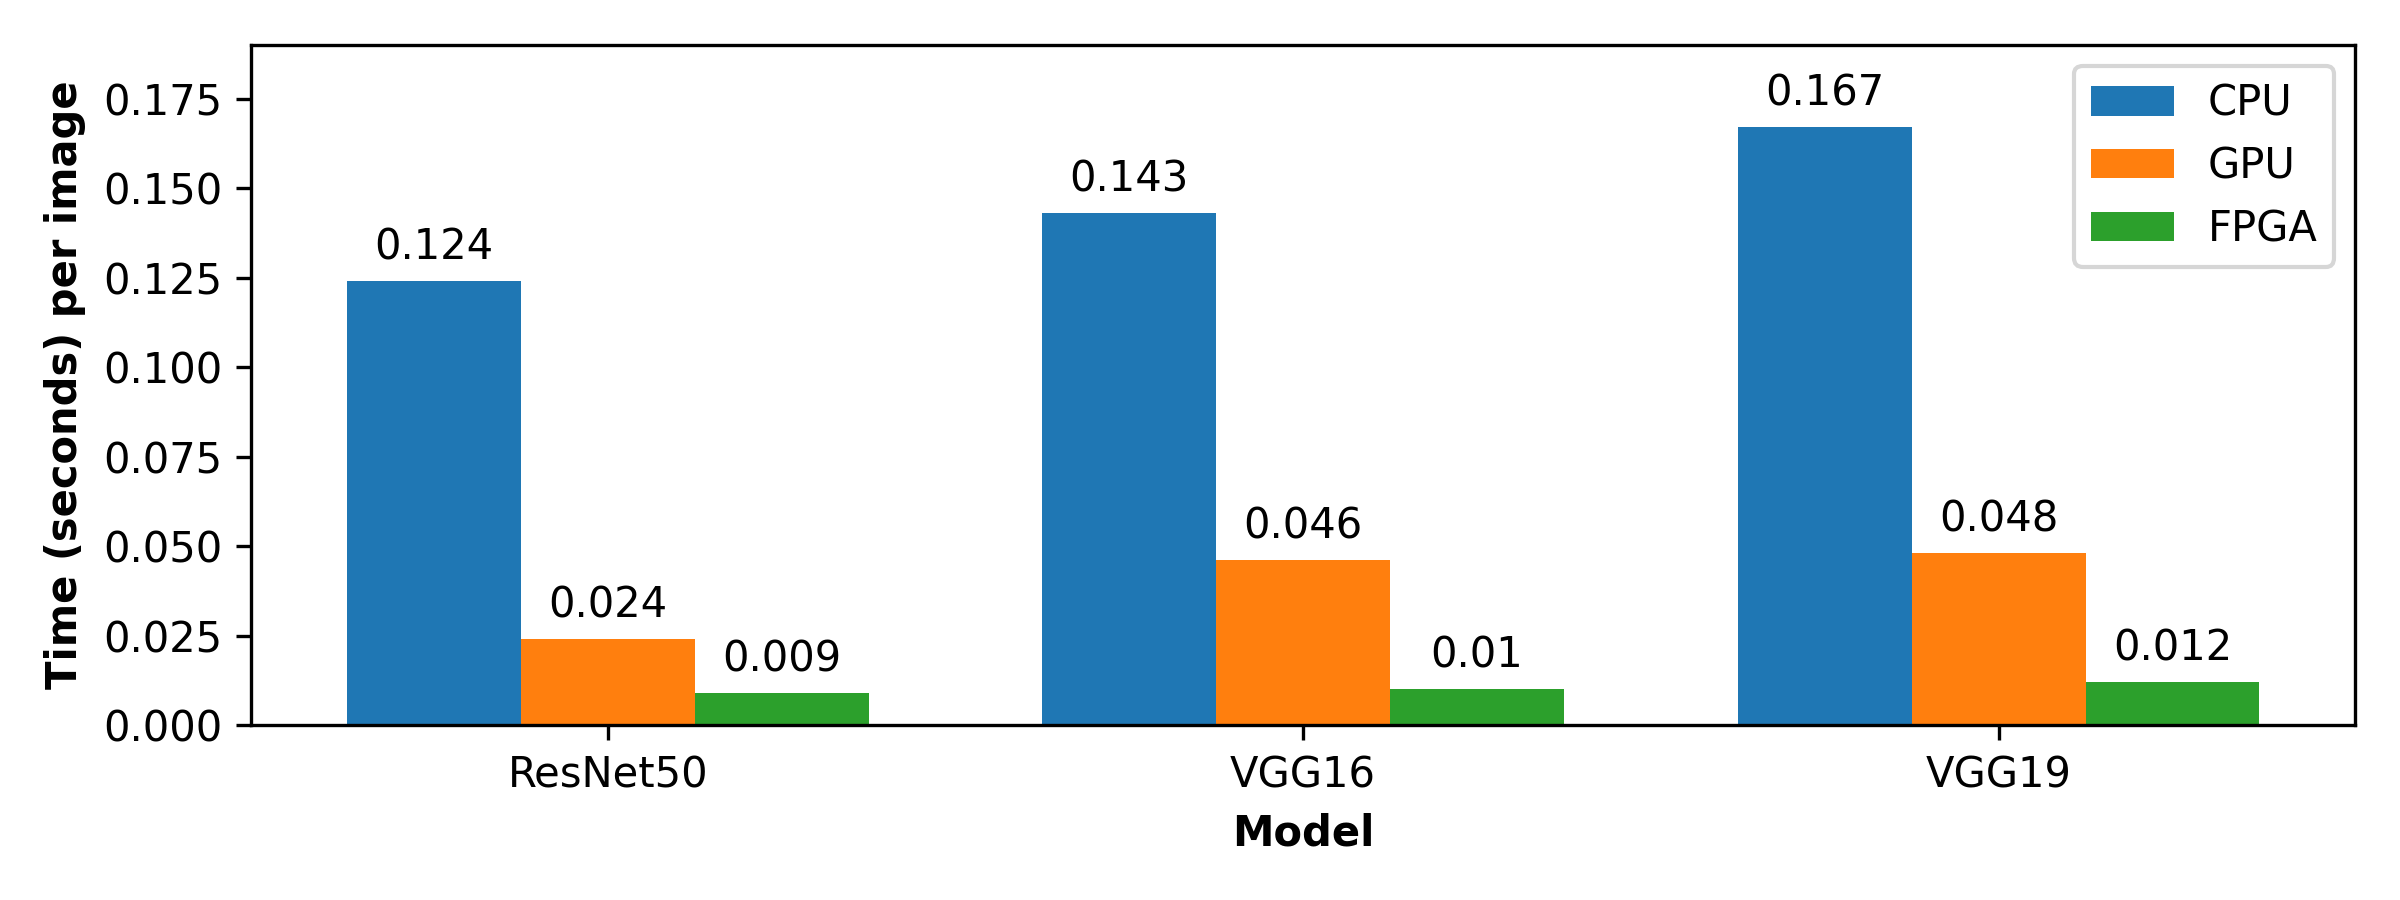
\includegraphics[width=\columnwidth]{4_Chapitre4/figures/characterization/time_of_inference_1_image.png}
\caption{Inference time for one image with ResNet50, VGG16 and VGG19.}
\label{figure:herofake-time-inference}
\end{figure}

La carte d'accélération FPGA étant censée être plus efficace qu'un CPU ou un GPU~\cite{5272532}, la comparaison du temps d'inférence avec ces trois technologies est une première condition pour permettre la comparaison du coût énergétique par image. L'évaluation des performances en termes de temps d'exécution a été réalisée avec les mêmes 10 000 images pour les trois modèles différents. Nous avons construit un ensemble de données deepfake à deux classes, les vraies provenant de l'ensemble de données CelebA~\cite{https://doi.org/10.48550/arxiv.1411.7766}, et les fausses générées à l'aide d'un Generative Adversarial Network (GAN)~\cite{jimaging7080128}. La quantification et la compilation du graphe ont été effectuées avec Vitis-AI afin de l'exécuter sur le FPGA. En ne considérant que le temps d'inférence, il s'est avéré que sur les trois modèles testés (ResNet50, VGG16 et VGG19), le FPGA est de 13,08 à 13,79 fois plus rapide que le CPU mais aussi de 2,52 à 4,48 fois plus rapide que le GPU (voir Figure~\ref{figure:herofake-time-inference}).

\subsection{Mesures de consommation d'énergie}

\begin{figure}[t]
\centering
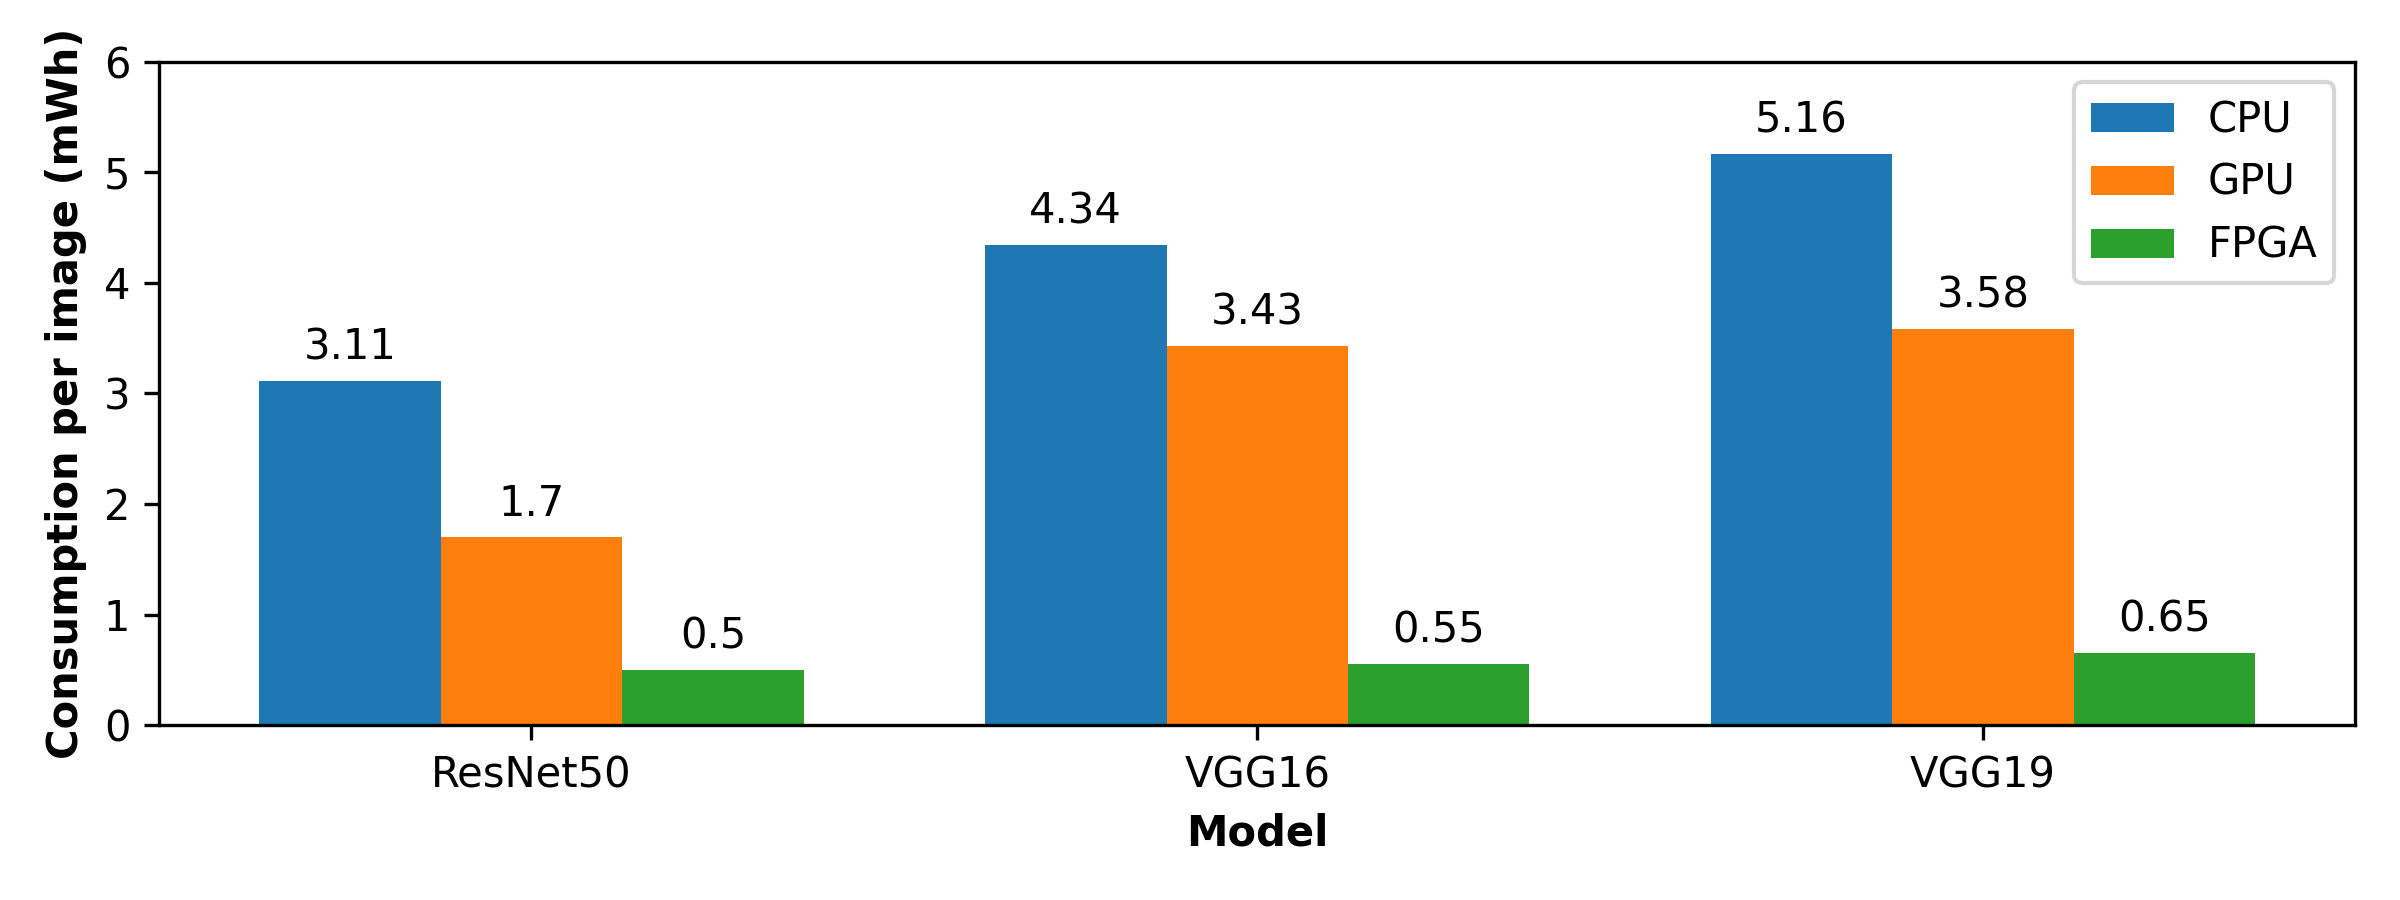
\includegraphics[width=\columnwidth]{4_Chapitre4/figures/characterization/consumption_per_image.png}
\caption{Energy consumption of inference per image (mWh).}
\label{figure:herofake-consumption-per-image}
\end{figure}

La consommation d'énergie instantanée mesurée pendant l'inférence est la consommation globale de la machine (y compris l'unité centrale, la mémoire, la carte mère et l'alimentation) pendant l'exécution de l'inférence. 
Les mesures ont été effectuées à l'aide d'une unité de distribution d'énergie (PDU) (Raritan PX3-5190R) capable de surveiller la puissance instantanée et la consommation d'énergie du serveur (Dell Precision T5810). Les résultats montrent que l'inférence sur le CPU produit la consommation d'énergie instantanée la plus faible. Ce résultat est assez attendu car l'inférence sur GPU ou FPGA inclut également la consommation d'énergie du CPU.


Cependant, la seule consommation d'énergie instantanée ne reflète pas correctement le coût total de chaque plateforme. Le temps d'exécution nécessaire pour traiter toutes les images doit être pris en compte. La mesure pertinente est le coût énergétique par image. La consommation d'énergie a été mesurée en kilowattheures (kWh) pour les 10 000 images, puis convertie en milliwattheures (mWh) par image. De ce point de vue, il est clair que le FPGA est le plus économe en énergie en ce qui concerne le temps d'exécution, consommant de 6,2 à 6,9 fois moins que le CPU et de 3,3 à 6,2 fois moins que le GPU (voir Figure~{figure:herofake-consumption-per-image}).

\subsection{Discussion}

\begin{figure}[t]
\centering
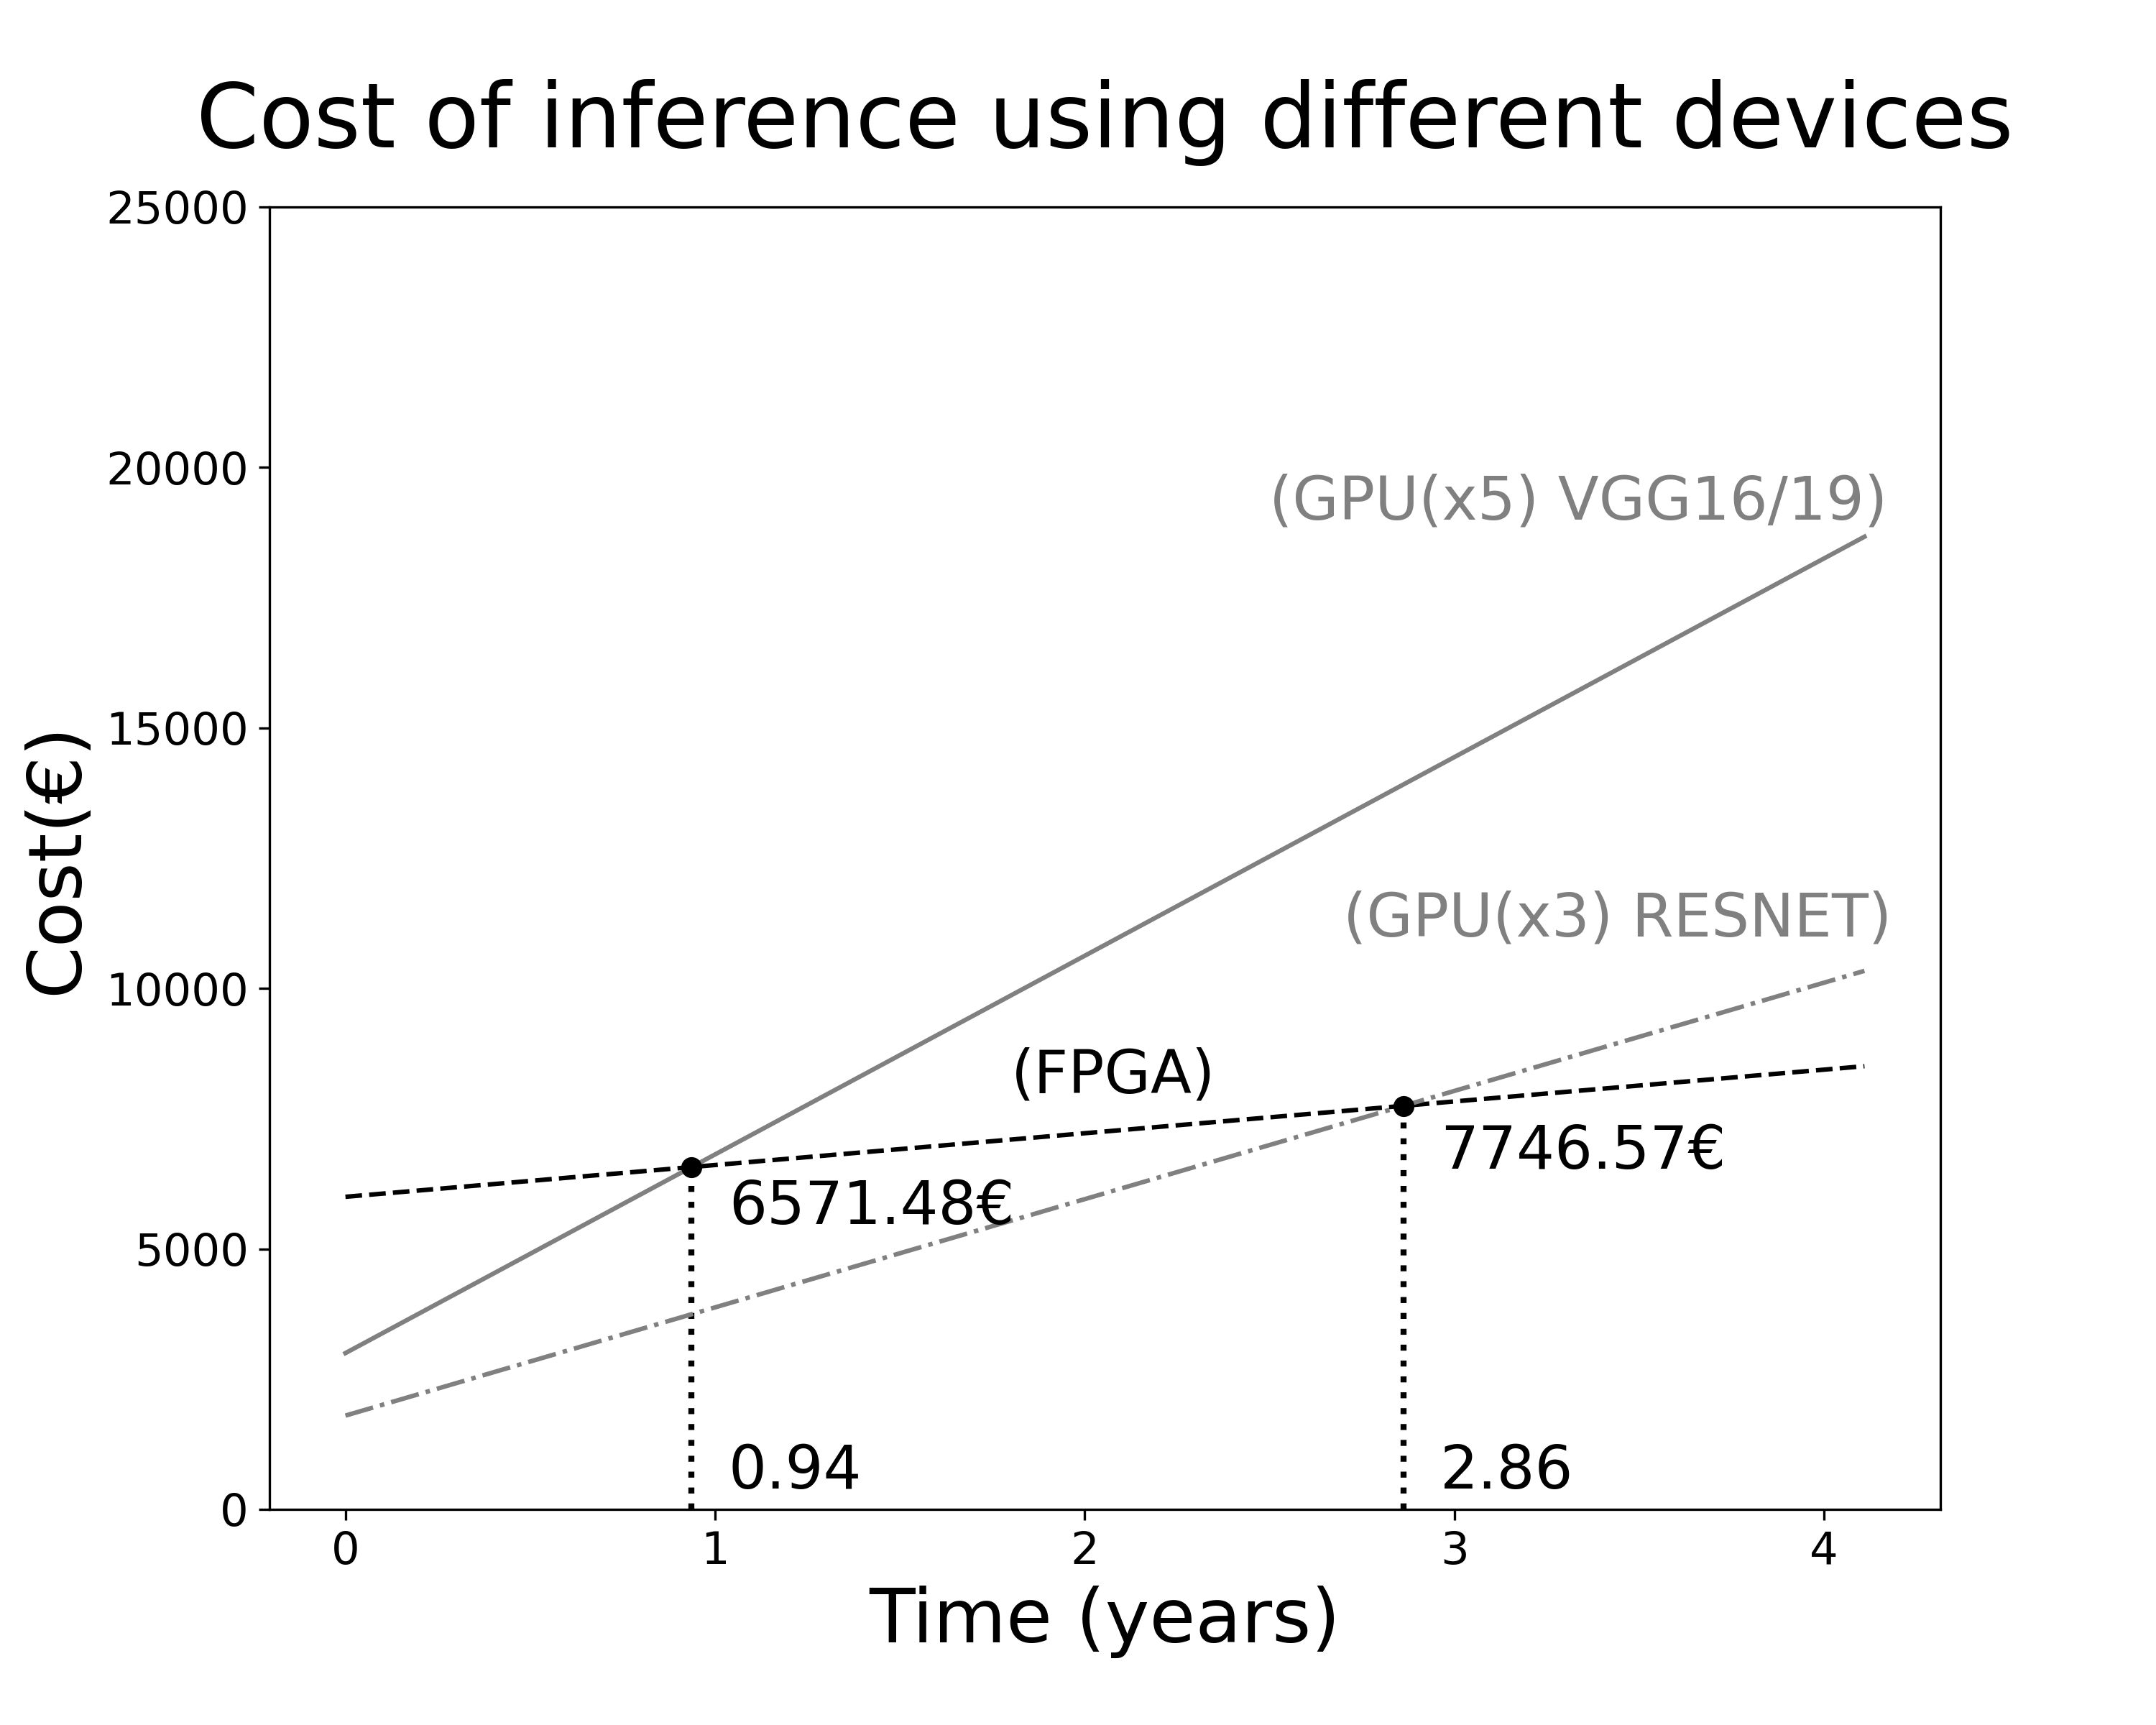
\includegraphics[scale=0.2]{4_Chapitre4/figures/characterization/cost_devices_time.png}
\caption{Total cost of inference on selected devices over time.}
\label{figure:herofake-cost-over-time}
\end{figure}

Les résultats de ce benchmark montrent un net avantage de l'inférence sur FPGA en termes de performance et d'efficacité énergétique. Les gains de performance sont significatifs, en particulier avec les réseaux d'apprentissage profond plus complexes~\cite{8782524}. Les ressources informatiques basées sur des serveurs équipés de cartes d'accélération FPGA, au lieu de cartes d'accélération GPU, bénéficieraient de ces avantages.

La consommation d'énergie brute du dispositif d'inférence ne reflète pas le coût total de la solution. En effet, il faut également inclure le coût de l'équipement lui-même. C'est un point important dans la comparaison entre GPU et FPGA, car il existe un écart de prix entre les deux technologies : le GPU (RTX 2070 Super) utilisé pour ce benchmark a été introduit aux alentours de 600€, alors que le FPGA (Alveo U250) est vendu aux alentours de 6000€. Le coût de l'énergie électrique pour effectuer l'inférence est très faible (nous avons utilisé la moyenne européenne de 0,1833 € par kWh proposée dans~\cite{energy-price}), comparé au coût initial du dispositif : la durée d'exécution nécessaire pour bénéficier de l'avantage de coût du FPGA est de l'ordre de plusieurs mois de fonctionnement continu. La figure~\ref{figure:herofake-cost-over-time} représente le coût cumulé (en euros) de l'utilisation d'un serveur avec accélération GPU ou FPGA en fonction du temps (en années). Notre estimation du coût comprend le nombre de GPU nécessaires et leur coût pour égaliser les performances des FPGA et utilise un facteur 2x~\cite{shehabiUnitedStatesData2016}, pour tenir compte de la consommation d'énergie totale de l'infrastructure (principalement le refroidissement et la mise en réseau). Le FPGA peut devenir une solution rentable après quelques mois pour les CNN complexes. Pour les réseaux moins complexes, l'avantage financier du FPGA est atteint après plus de deux ans.

\begin{figure}[t]
\centering
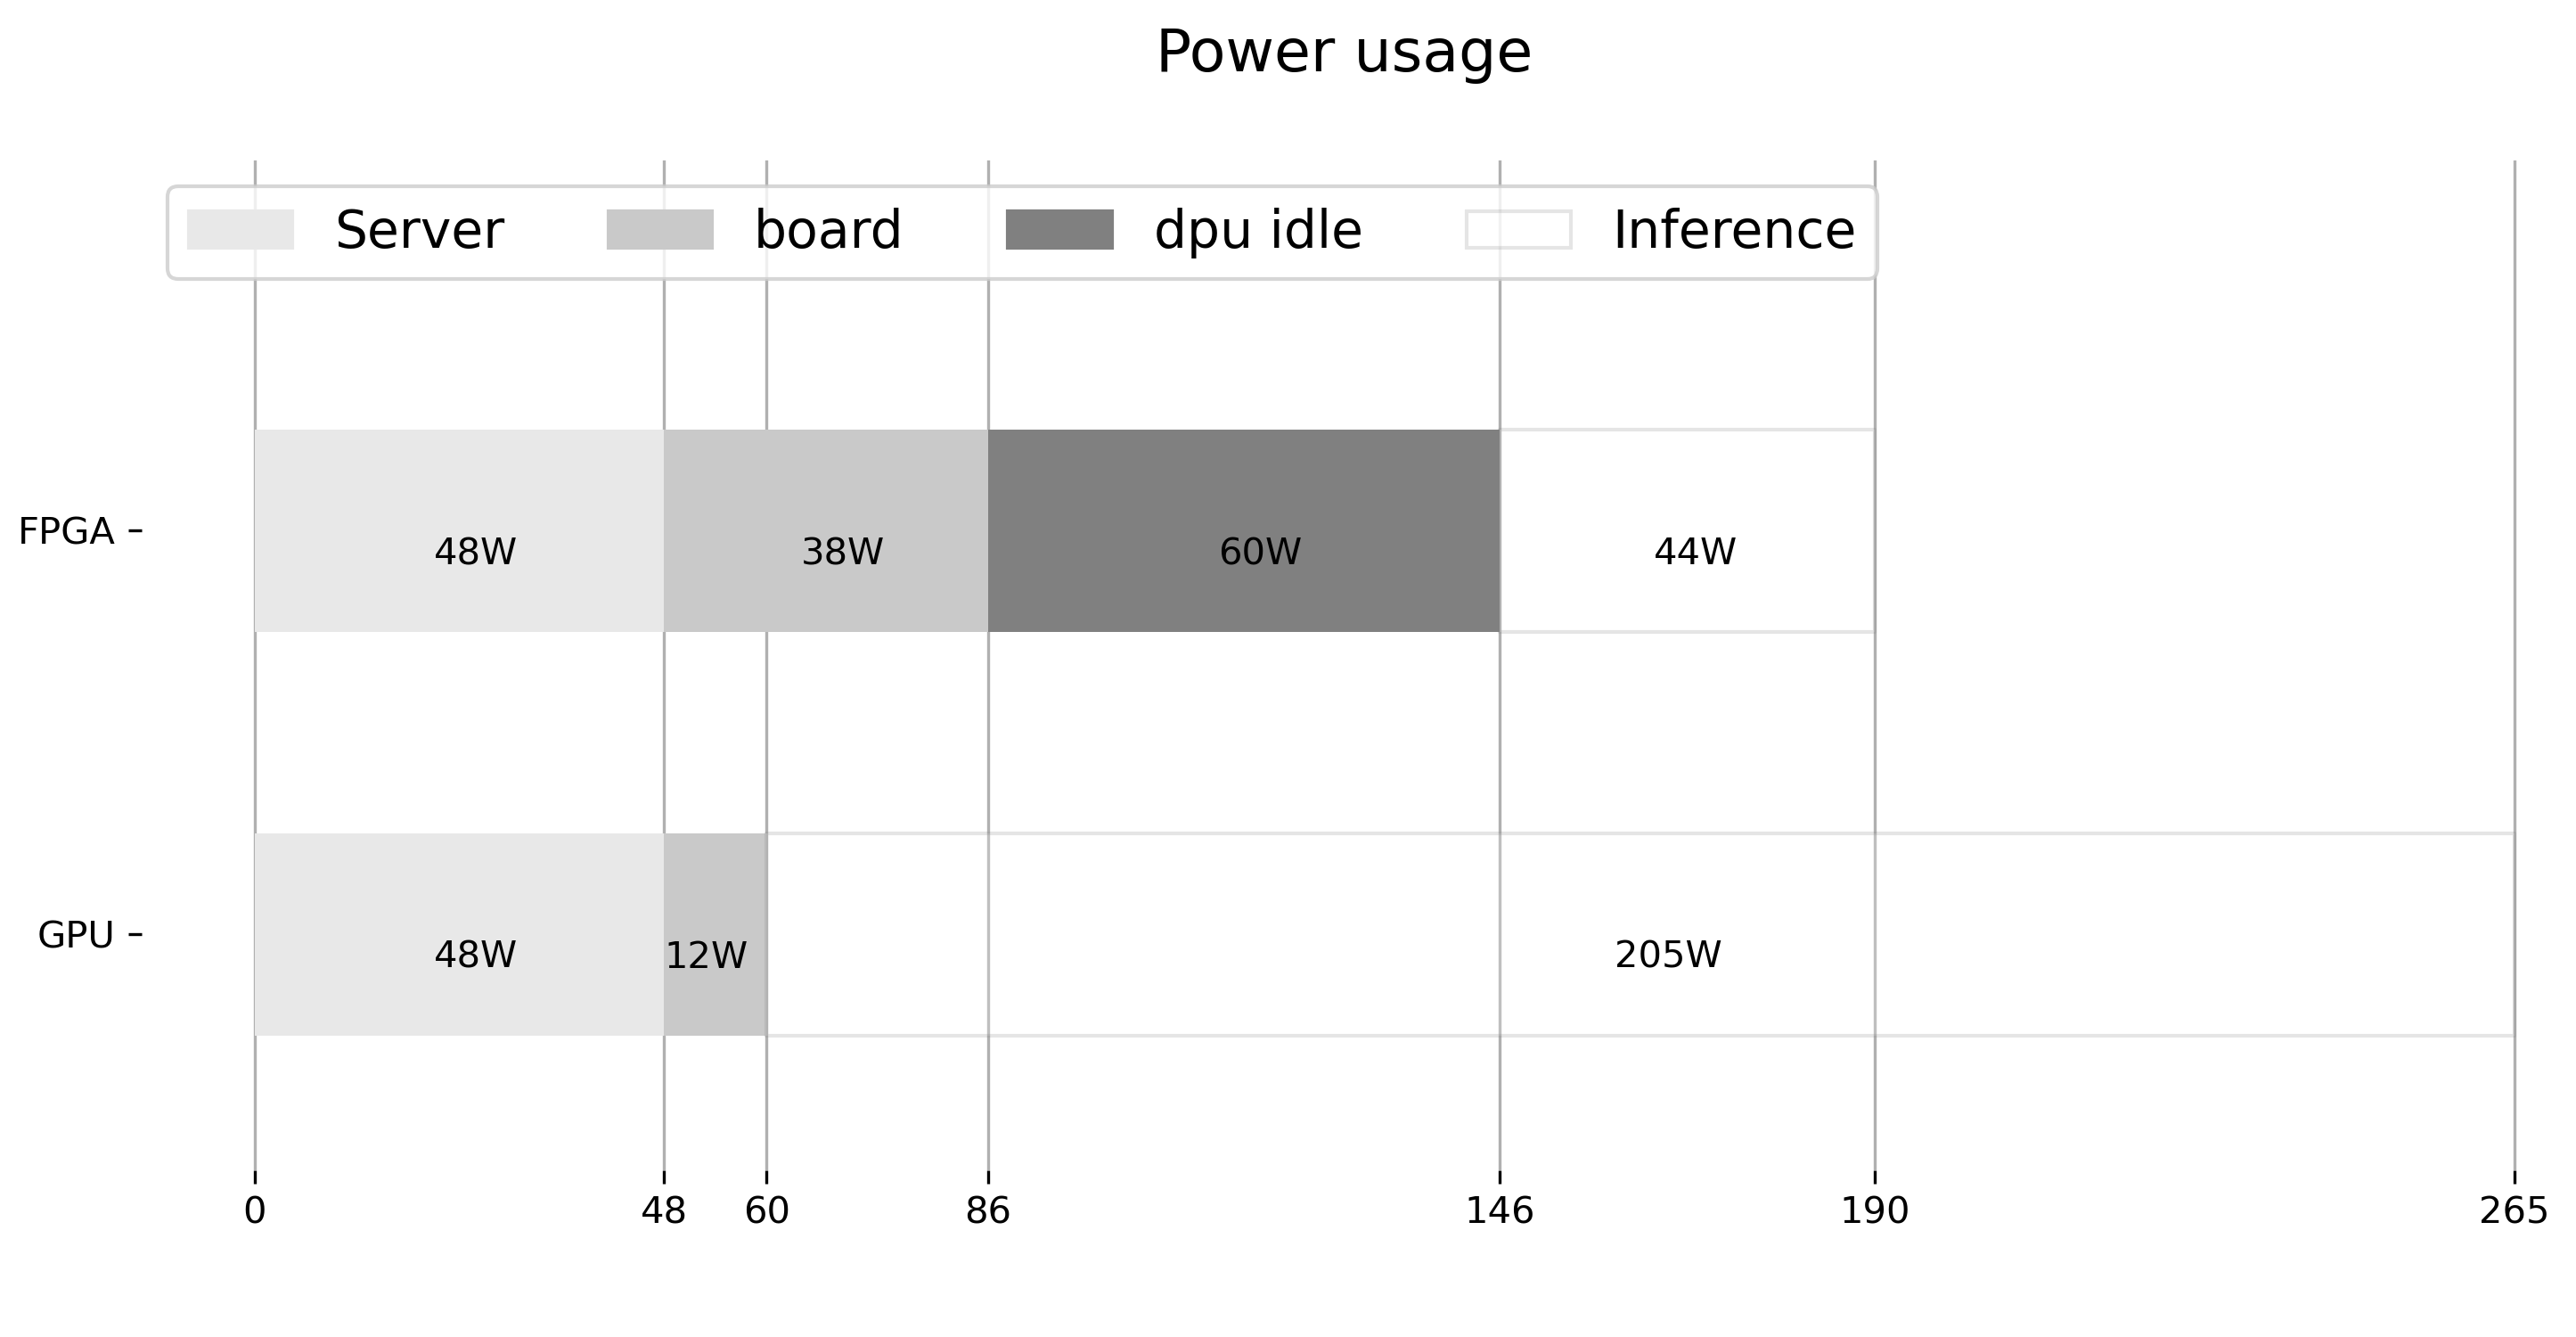
\includegraphics[width=\columnwidth]{4_Chapitre4/figures/characterization/power_usage.png}
\caption{Power usage breakdown for FPGA and GPU.}
\label{figure:herofake-power-usage}
\end{figure}

L'analyse précédente est valable dans le cas où l'inférence est toujours effectuée à pleine charge. En effet, lorsque l'on décompose la consommation d'énergie du GPU entre la consommation au repos et la consommation pour l'inférence, il est clair que le GPU est capable d'adapter dynamiquement sa consommation d'énergie à l'intensité du traitement. Le FPGA, quant à lui, semble avoir une gestion de l'énergie très limitée. Une fois que la conception du DPU est chargée dans le dispositif, sa consommation d'énergie au repos reste très élevée (voir la figure. \ref{figure:herofake-power-usage}). Si l'on ajoute les 38 W de la carte FPGA, il y a en effet une consommation résiduelle de 60 W lorsque le DPU est inactif. Même si l'évolution de l'implémentation du DPU sur le FPGA peut résoudre ce problème (par exemple en réduisant l'activité de l'arbre d'horloge lorsqu'il est inactif), cela a un impact sur le coût total et doit être pris en compte si le dispositif n'est pas toujours utilisé à pleine charge. Avec seulement 12 W d'énergie au repos, le GPU est un meilleur candidat lorsque l'utilisation à pleine charge du dispositif ne peut être garantie.

Comme la tendance vers des CNN plus complexes se poursuit~\cite{8807741}, l'utilisation des dispositifs les plus efficaces deviendra un défi majeur. La solution FPGA offre une nouvelle option pour effectuer l'inférence. Cependant, les FPGA ne remplacent pas encore les GPU : le flux de compilation reste complexe et prend du temps. Il faudra trouver un compromis entre la flexibilité des GPU et l'efficacité des FPGA. La section suivante traite d'un premier orchestrateur qui prend en compte la caractérisation mentionnée ci-dessus pour l'allocation et l'ordonnancement de ressources hétérogènes.

\section{Phase en ligne : allocation des ressources et placement des tâches}
\label{section:herofake-online}

Dans cette section, nous formulons le problème que notre contribution aborde, et nous donnons une description détaillée de notre modèle. Enfin, nous présentons une description formelle de notre stratégie pour la mise à l'échelle automatique des ressources et l'ordonnancement des tâches. 

\subsection{Défis pour l'orchestration dynamique}

L'ordonnancement des charges de travail dans le paradigme serverless est un problème à deux volets : les fournisseurs doivent gérer dynamiquement l'allocation des ressources (c'est-à-dire gérer les pools de ressources lors de la mise à l'échelle du nombre de répliques pour une application) et le placement des tâches (c'est-à-dire le mappage des tâches aux répliques existantes).

L'augmentation du nombre de répliques pose un problème de performance : lorsqu'une nouvelle réplique est créée, que ce soit sous la forme d'un conteneur ou d'une machine virtuelle, le bac à sable d'exécution doit passer par sa phase d'initialisation. C'est ce qu'on appelle un "démarrage à froid".

Les solutions commerciales telles que AWS Lambda évitent souvent le problème du démarrage à froid en maintenant des pools de bacs à sable préchauffés~\cite{vahidiniaColdStartServerless2020}. Ces machines virtuelles (VM) ou conteneurs sont démarrés par anticipation et mis en pause dans un état post-initialisation. Lorsque l'activité reprend, les demandes entrantes peuvent être servies sans souffrir d'un délai de démarrage à froid, au détriment du multiplexage des ressources du côté du fournisseur. Bien que cette solution permette de réduire, voire d'éliminer les délais de démarrage à froid, elle pèse sur la capacité de multiplexage des ressources du fournisseur et augmente le coût total de possession (TCO).

En outre, les applications de Machine Learning as a Service (MLaaS) présentent une charge très fluctuante~\cite{gujaratiSwayamDistributedAutoscaling2017}, ce qui renforce l'argument selon lequel une stratégie d'allocation des ressources réactive est nécessaire pour redimensionner l'infrastructure. Cependant, comme le temps d'exécution des tâches d'inférence est de l'ordre du centième ou du dixième de seconde, tandis que le temps d'initialisation des bacs à sable peut aller du centième de seconde à la seconde~\cite{mancoMyVMLighter2017}, nous avons besoin d'un mécanisme pour éviter d'encourir d'énormes coûts de latence pour l'exécution des fonctions.

Les tâches critiques nécessitent des garanties de niveau de service de la part du fournisseur. Les accords de niveau de service dans le cloud consistent généralement à convenir d'un taux de disponibilité des ressources dans le temps ; si le fournisseur ne respecte pas cet accord, une remise est proposée au client. Bien que cela puisse fonctionner pour des ressources réservées, nous pouvons voir que cela n'a pas de sens dans le paradigme serverless. La possibilité de garantir le temps de réponse des tâches permettrait à un fournisseur serverless d'atteindre des accords de niveau de service par invocation~\cite{zhangMArkExploitingCloud}.

L'utilisation d'accélérateurs matériels est une possibilité d'améliorer les rapports performance-coût. Bien qu'il s'agisse d'un investissement coûteux (voir Figure~\ref{figure:herofake-cost-over-time}), ces dispositifs permettent d'accélérer considérablement les tâches parallèles (voir Figure~\ref{figure:herofake-time-inference}), améliorant ainsi le temps de réponse des fonctions, avec un coût énergétique réduit (voir Figure~\ref{figure:herofake-consumption-per-image}).

\subsection{Modèle de tâche} \label{model:tasks}

\begin{table}[t]
    \caption{Notation dictionary}
    \begin{center}
    \begin{tabular}{|c|L|}
    \hline
    \textbf{Notation} & \textbf{Description} \\ \hline
    $f_{N, P}$ & A function $f$ scheduled to run on a platform $P$ available on node $N$ \\ \hline
    $QP$ & QoS penalty \\ \hline
    $QD$ & QoS deviation \\ \hline
    $WET$ & Worst execution time \\ \hline
    $TT$ & Task total time \\ \hline
    $WT$ & Wait time \\ \hline
    $CST$ & Cold start time \\ \hline
    $ET$ & Execution time \\ \hline
    $EC$ & Energy consumption \\ \hline
    $HP$ & Hardware price \\ \hline
    $TC$ & Task consolidation \\ \hline
    $Q$ & Task queue on a replica \\ \hline
    $replicaCount_{f}$ & Size of the replica pool in the system for a function $f$ \\ \hline
    $concurrency_{f}$ & Average number of in-flight requests for a function $f$ \\ \hline
    $threshold$ & Concurrency threshold for function replicas in vanilla Knative \\ \hline
    $replicaCount_{f, h}$ & Size of the replica pool for a function $f$ on hardware type $h$ \\ \hline
    $concurrency_{f, h}$ & Average number of in-flight requests for a function $f$ on replicas of hardware type $h$ \\ \hline
    $x_{f, h}$ & Concurrency threshold for a function $f$ on a replica of hardware type $h$ \\ \hline
    $scaleCost_{{f}_{N, P}}$ & Cost of creating a new replica for function $f$ on a platform $P$ available on node $N$ \\ \hline
    $schedCost_{{f}_{N, P}}$ & Cost of scheduling an execution of function $f$ on a platform $P$ available on node $N$ \\ \hline
    \end{tabular}
    \label{table:herofake-notation}
    \end{center}
\end{table}

Les applications sont composées de fonctions. L'exécution d'une fonction est appelée \textit{tâche}. Dans ce travail, il n'y a pas de dépendances entre ces tâches : l'application est composée de fonctions pures et sans état. Les événements qui déclenchent l'exécution d'une tâche arrivent dans le système à un intervalle aléatoire et borné. Nous formulons l'hypothèse qu'une requête aboutit toujours et conduit à l'exécution d'une \textit{task} (une instance de \textit{fonction}). Lorsqu'une tâche a commencé son exécution sur la plateforme qui lui a été attribuée, elle s'exécute pendant la totalité de son temps d'exécution. Nous ne prenons pas en compte la préemption ou les défaillances dans cette contribution : une tâche termine toujours son exécution avec succès, même si son temps de réponse peut dépasser ses exigences en matière de qualité de service. Nous ne tenons pas compte des interférences possibles entre les charges de travail sur le même nœud~\cite{dartoisInvestigatingMachineLearning2021}. 

Nous considérons les tâches qui peuvent être exécutées sans distinction sur des plateformes d'exécution hétérogènes. Dans le contexte de notre étude de cas spécifique, la mise en œuvre des différentes fonctions a été effectuée à la main pour chaque plateforme ; cependant, des travaux existent pour permettre une compilation croisée automatique pour les architectures hétérogènes~\cite{hortaXartrekRuntimeExecution2021, 10.1145/3445814.3446699}. Les métadonnées suivantes ont été mesurées pour chaque fonction, sur chaque plateforme d'exécution : 

\begin{itemize}
    \item \textit{Besoins mémoire en pic} -- la quantité de mémoire (en GB) allouée à la tâche ;
    \item \textit{Durée de démarrage à froid} -- la durée de l'initialisation du bac à sable lors de l'exécution de la tâche sur une plateforme qui n'a pas la fonction en cache ;
    \item \textit{Temps d'exécution} -- la durée prévue de l'exécution effective de la tâche, à l'exclusion de sa phase d'initialisation ;
    \item \textit{Consommation d'énergie} -- la différence entre l'énergie inactive et l'énergie active encourue par la plateforme d'exécution lorsqu'elle exécute la tâche.
\end{itemize}

L'équation~\ref{eq:herofake-HRO-total-time} décompose le temps de réponse attendu pour l'exécution d'une fonction $f$ sur une plateforme $P$ sur un nœud $N$.

\begin{equation}
    {TT}_{{f}_{N, P}} = {WT}_{{f}_{N, P}} + {CST}_{{f}_{N, P}} + {ET}_{{f}_{N, P}}
\label{eq:herofake-HRO-total-time}
\end{equation}

Où :

\begin{itemize}
    \item ${WT}_{{f}_{N, P}}$ correspond à la durée de la décision d'ordonnancement, y compris le temps passé par la requête en file d'attente ;
    \item ${CST}_{{f}_{N, P}}$ est la durée de l'initialisation de l'invocation de la fonction, y compris son temps potentiel de démarrage à froid ;
    \item ${ET}_{{f}_{N, P}}$ est le temps d'exécution de la fonction sur la plateforme.
\end{itemize}

Nous proposons différents niveaux de qualité de service en fonction des besoins des utilisateurs en termes de garanties sur le temps d'exécution. Chaque niveau de qualité de service présente un \textit{écart de durée} différent (noté $QD$ dans l'équation~\ref{eq:herofake-task-penalty}) -- un facteur par lequel le pire temps d'exécution d'une fonction est multiplié pour donner une limite supérieure au temps d'exécution de cette fonction pour ce niveau de qualité de service.

Le temps d'exécution prédit d'une fonction est toujours basé sur le pire temps d'exécution (noté $WET_{f}$), c'est-à-dire le temps d'exécution d'une tâche lorsqu'elle est programmée sur la plateforme d'exécution présentant le niveau de performance le plus faible pour cette fonction :


\begin{equation}
    \forall \, (N, P), \, WET_{f} = \max ET_{N, P}
\label{eq:herofake-task-wet}
\end{equation}

Une fois qu'une tâche est programmée sur une plateforme d'exécution, elle passe par sa durée totale d'exécution décrite dans l'équation \ref{eq:herofake-HRO-total-time}. L'échéance de la tâche est calculée en multipliant le pire temps de réponse de la fonction (tel qu'exprimé dans l'équation~\ref{eq:herofake-task-wet}) par l'écart de durée de la qualité de service associé au niveau de qualité de service de la demande de l'utilisateur. L'équation~\ref{eq:herofake-task-penalty} montre que nous fixons une valeur booléenne $QP_{f_{N, P}}$ pour chaque invocation de fonction si la tâche ne respecte pas son délai. 


\begin{equation}
    QP_{f_{N, P}} = TT_{f_{N, P}} \cdot QD_{f_{N, P}} > WET_{f}
\label{eq:herofake-task-penalty}
\end{equation}

\subsection{Stratégie d'allocation de ressources} \label{section:herofake-autoscaling-strategy}

Dans une plateforme serverless, l'autoscaler a la responsabilité d'allouer des ressources matérielles pour les exécutions de fonctions. Pour toute fonction, un autoscaler peut allouer $n$ \textit{répliques}. Le nombre de répliques pour une fonction donnée à un moment donné détermine le niveau de concurrence.

Dans Knative, le nombre de répliques pour une fonction donnée (équation~\ref{eq:herofake-kn-replica-count}) dépend de la charge moyenne mobile pour une fonction, c'est-à-dire le nombre moyen de requêtes en vol pour la fonction sur une fenêtre de 60 secondes (concurrence dans le système par fonction). Il est limité par un seuil de concurrence par réplique, c'est-à-dire le nombre maximum de demandes en file d'attente dans la réplique d'une fonction à tout moment. La valeur par défaut dans Knative est de 100 requêtes en vol dans chaque réplique~\cite{knative-autoscaling}.

\begin{equation}
    replicaCount_{f} = \frac{concurrency_{f}}{threshold}
\label{eq:herofake-kn-replica-count}
\end{equation}

Ce mécanisme de dimensionnement permet d'allouer des CPU sous Knative, en réaction aux changements de l'état actuel de la concurrence dans le système. La principale contribution de l'autoscaler que nous proposons est d'améliorer Knative afin de prendre en compte l'hétérogénéité des plateformes d'exécution.

Le mécanisme Knative simple ne fonctionne pas lorsque l'infrastructure est constituée d'une variété de plateformes d'exécution. En effet, ces plateformes présentent différents niveaux de performance, de consommation d'énergie et de coût. Cela a une conséquence sur le nombre de répliques que le fournisseur doit déployer sur ces plateformes : pour un niveau donné de charge d'application, les répliques hétérogènes seront capables de traiter différents nombres de tâches dans le même délai. Pour que notre plateforme puisse gérer l'hétérogénéité de l'infrastructure sous-jacente, nous proposons un nombre de répliques par fonction et \textbf{par type de matériel} comme dans l'équation~\ref{eq:herofake-HRO-replica-count}.

\begin{equation}
    replicaCount_{f, h} = \frac{concurrency_{f, h}}{x_{f, h}}
\label{eq:herofake-HRO-replica-count}
\end{equation}

Une décision d'autoscaling peut introduire des coûts d'opportunité dans le système : les accélérateurs matériels sont peu disponibles par rapport aux CPU, et le fait de les allouer à une fonction donnée à un moment donné les rendra indisponibles pour d'autres calculs. Pour que l'autoscaler puisse décider quand il est pertinent d'allouer de tels accélérateurs, il doit être conscient des coûts. 

Afin de déterminer le seuil de concurrence par réplique $x_{f, h}$ pour une fonction $f$ sur un type de matériel $h$ (par exemple, GPU et FPGA), nous avons fixé le seuil de concurrence par réplique sur les CPU à $x_{f, c} = 100$, comme c'est la valeur par défaut dans Knative~\cite{knative-concurrency}. Ensuite, nous avons utilisé les mesures de la phase hors-ligne (Table~\ref{table:herofake-tasks}) pour établir un ratio composite (incluant la performance, l'énergie, le prix de la plateforme) comme décrit dans l'équation~\ref{eq:herofake-HRO-concurrency-target}. Dans notre politique, nous avons choisi de favoriser le temps de réponse en fixant $k_{ET} = \frac{2}{3}$, $k_{EC} = \frac{1,5}{6}$ et $k_{HP} = \frac{0,5}{6}$. Par exemple, pour la fonction ResNet50 (décrite dans Table~\ref{model:tasks}), les files d'attente de tâches dans les réplicas sont dimensionnées à 100 pour les CPU, 489 pour les GPU et 1292 pour les FPGA.

\begin{equation}
    x_{f, h} = x_{f, c} \cdot (k_{ET} \cdot \frac{ET_{{f}_{c}}}{ET_{{f}_{h}}} + k_{EC} \cdot \frac{EC_{{f}_{c}}}{EC_{{f}_{h}}} + k_{HP} \cdot \frac{HP_{{f}_{c}}}{HP_{{f}_{h}}})
\label{eq:herofake-HRO-concurrency-target}
\end{equation}

Lorsque le seuil de simultanéité d'une fonction est dépassé dans les files d'attente des répliques sur un type de matériel donné, l'autoscaler procède à la \textit{scale out} de la fonction : une nouvelle réplique est mise en route pour traiter les demandes ultérieures des utilisateurs.

L'allocation commence par la liste complète des nœuds disponibles dans l'infrastructure. Nous commençons par constituer un sous-ensemble de nœuds disponibles, appelé \textit{nœuds appropriés}. Compte tenu des besoins en mémoire que nous avons mesurés pour chaque fonction, nous éliminons les nœuds qui ne disposent pas actuellement de suffisamment de mémoire pour exécuter une réplique de la fonction. Chaque réplique déployée sur la plateforme d'exécution d'un nœud consomme la quantité totale de mémoire requise par le type de fonction. Si le nœud n'a plus de mémoire, ses plateformes d'exécution ne peuvent plus être utilisées pour déployer d'autres répliques.

Afin de sélectionner le type de ressource à allouer à cette réplique, l'autoscaler minimise la fonction de coût donnée dans l'équation~\ref{eq:herofake-HRO-allocation-cost-function}. 
Dans notre politique, comme pour l'autoscaling, nous avons choisi de favoriser le temps total d'exécution des tâches en fixant $k_{TT} = \frac{2}{3}$, $k_{EC} = \frac{1.5}{6}$ et $k_{HP} = \frac{0.5}{6}$. 
En fonction du matériel disponible dans le pool au moment de la mise à l'échelle, l'autoscaler favorisera la création d'une nouvelle réplique de fonction sur la plateforme qui exécutera la tâche dans le temps total le plus court, y compris le démarrage à froid, avec la consommation d'énergie la plus faible et le prix le plus bas.

\begin{equation}
\begin{split}
    scaleCost_{{f}_{N, P}} = \, &k_{TT} \cdot {TT}_{{f}_{N, P}} \\
    + &k_{EC} \cdot {EC}_{{f}_{N, P}} \\
    + &k_{HP} \cdot {HP}_{{f}_{N, P}}
\end{split}
\label{eq:herofake-HRO-allocation-cost-function}
\end{equation}

Au contraire, lorsque la concurrence pour une fonction tombe en dessous du seuil sur un type de matériel donné, l'autoscaler emploiera une politique de meilleur effort et essaiera de désallouer tout réplica avec une file d'attente de tâches vide sur ce type de matériel. Si une réplique a une file d'attente de tâches vide, elle sera libérée dans le pool de plates-formes disponibles et la mémoire qui lui avait été allouée sur le nœud sera libérée.

Les différents poids ($k$) utilisés dans les équations~\ref{eq:herofake-HRO-concurrency-target} et~\ref{eq:herofake-HRO-allocation-cost-function} peuvent être modifiés par le fournisseur afin de personnaliser la politique d'allocation en fonction de différentes priorités.

\subsection{Stratégie d'ordonnancement} \label{section:herofake-scheduling-strategy}

La caractérisation de la charge de travail est essentielle à la prédiction des performances, car elle peut guider les décisions d'ordonnancement qui conduisent à la satisfaction des exigences de qualité de service~\cite{mampageHolisticViewResource2022}. Notre stratégie d'ordonnancement s'appuie sur les métadonnées des tâches décrites dans la section~\ref{model:tasks}. La construction de connaissances sur les tâches serverless est réalisée au cours d'une phase hors-ligne sur notre plateforme, car le code est poussé vers les registres du fournisseur avant l'exécution réelle~\cite{shahradServerlessWildCharacterizing}.

Dans Knative, le planificateur gère les tâches entrantes de manière FIFO. Pour gérer les différents niveaux d'exigences en matière de qualité de service, nous proposons que notre ordonnanceur retire les tâches de la file d'attente de l'orchestrateur par \textbf{échéance la plus proche}. Nous calculons l'échéance de la tâche en utilisant sa pire durée d'exécution sur la plateforme à l'aide de l'équation~\ref{eq:herofake-task-wet}, et en la multipliant par l'écart de durée autorisé fixé par le niveau de qualité de service. Après l'exécution de la tâche, nous vérifierons si nous avons dépassé son échéance et fixerons la pénalité associée en conséquence, comme décrit dans l'équation~\ref{eq:herofake-task-penalty}. 

Nous itérons sur les répliques de la fonction pour récupérer et prédire les métriques suivantes basées sur les métadonnées de la tâche :

\begin{itemize}
    \item \textbf{pénalité potentielle} : nous calculons la longueur de la file d'attente de la plateforme et vérifions si l'échéance de la tâche sera dépassée, comme décrit dans l'équation~\ref{eq:herofake-task-penalty} ;
    \item \textbf{consommation d'énergie} : nous récupérons les mesures hors-ligne pour établir la consommation d'énergie dynamique de cette tâche sur la plateforme ;
    \item \textbf{fusion des tâches} : nous calculons la longueur de la file d'attente des tâches de la plateforme $Q$ en additionnant les durées totales de toutes les tâches en file d'attente, comme décrit dans les équations~\ref{eq:herofake-HRO-scheduling-platform-queue} (longueur de la file d'attente) et~\ref{eq:herofake-HRO-total-time} (durée totale de la tâche). 
\end{itemize}

\begin{equation}
    len \, Q_{N, P} = \sum TT_{f_{N, P}}
\label{eq:herofake-HRO-scheduling-platform-queue}
\end{equation}

Ces valeurs sont normalisées pour s'adapter à une fonction de coût pondérée décrite dans l'équation~\ref{eq:herofake-HRO-scheduling-cost-function}. Nous avons utilisé $k_{QP} = \frac{2}{3}$, $k_{EC} = \frac{0.5}{6}$ et $k_{TC} = \frac{1.5}{6}$ (comme pour l'autoscaler). L'ordonnanceur minimise ensuite cette fonction de coût pour toutes les répliques $(N, P)$ (c'est-à-dire le nœud et la plateforme d'exécution).

\begin{equation}
\begin{split}
    schedCost_{{f}_{N, P}} = \, &k_{QP} \cdot QP_{{f}_{N, P}} \\
    + &k_{EC} \cdot {EC}_{{f}_{N, P}} \\
    + &k_{TC} \cdot TC_{{f}_{N, P}}
\end{split}
\label{eq:herofake-HRO-scheduling-cost-function}
\end{equation}

Si l'ordonnanceur ne trouve pas de réplique disponible pour exécuter la tâche, celle-ci sera repoussée dans la file d'attente de l'orchestrateur. Cela augmentera la concurrence dans le système pour la fonction, poussant l'autoscaler à allouer une autre réplique sur le matériel approprié.

\section{Évaluation}
\label{section:herofake-evaluation}

\begin{figure*}[t]
    \centering
    \subfloat[Task consolidation (based on the unused node count)\label{figure:herofake-evaluation-full-nodes}]{
        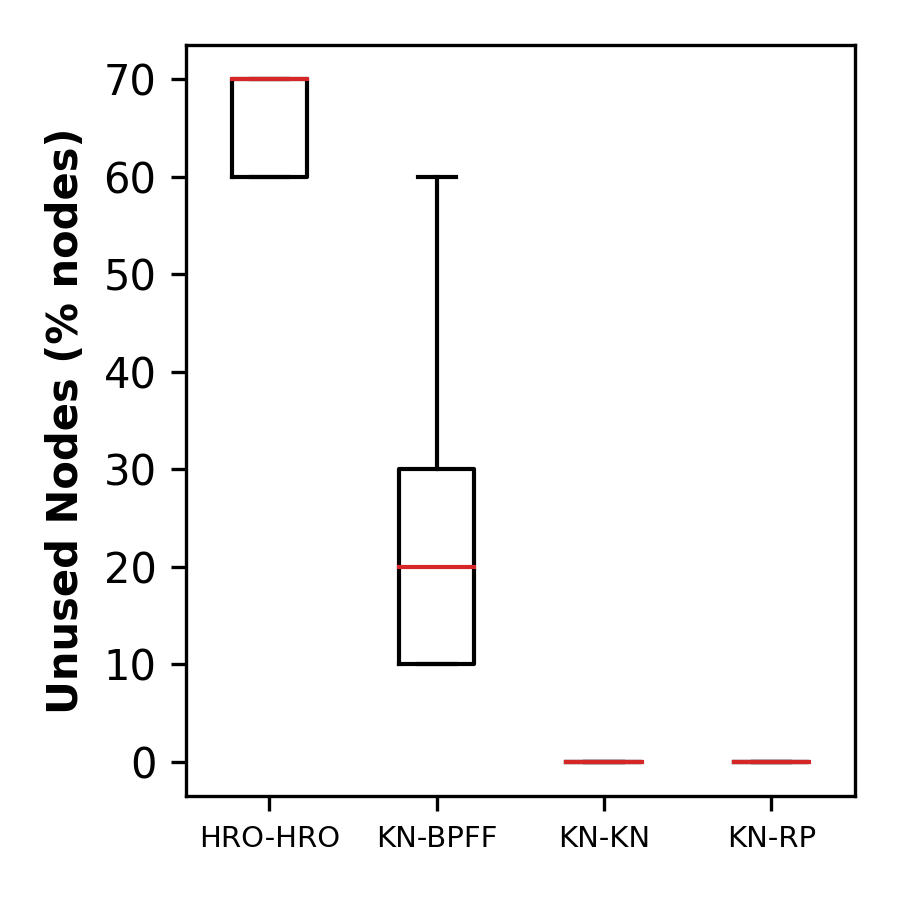
\includegraphics[width=0.28\linewidth]{4_Chapitre4/figures/evaluation/z-nodes-20221212-232143-169224.png}
    }\qquad
    \subfloat[QoS violations (based on tasks with missed deadline)\label{figure:herofake-evaluation-full-penalty}]{
        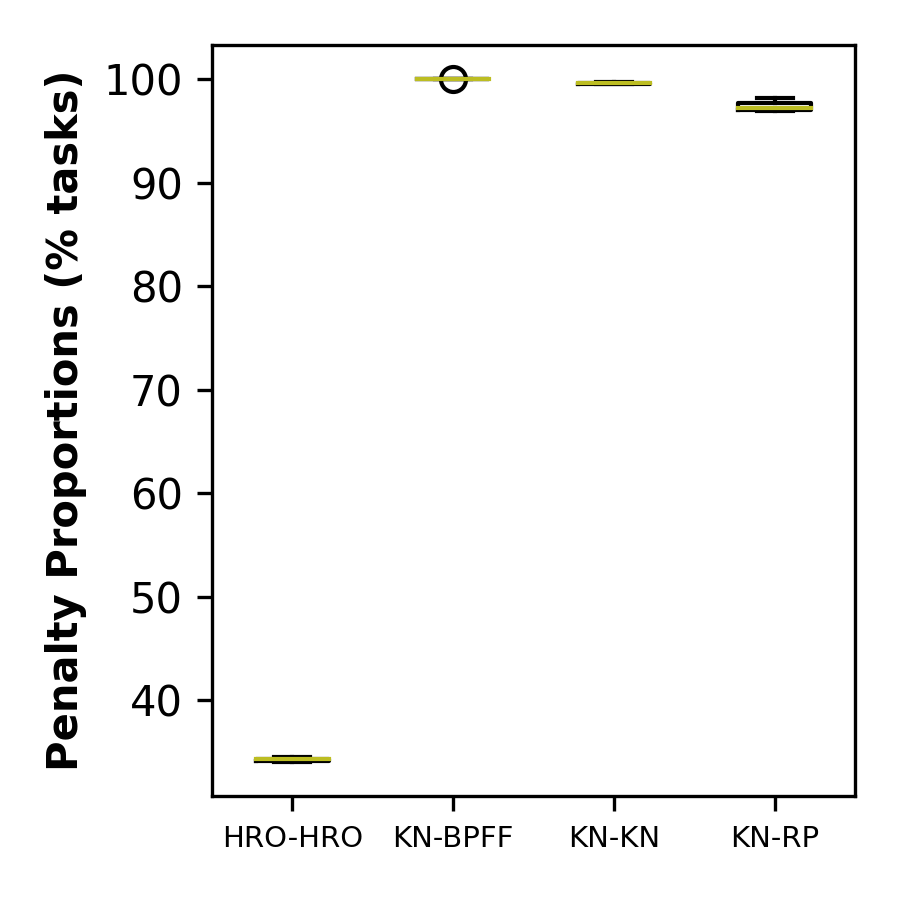
\includegraphics[width=0.28\linewidth]{4_Chapitre4/figures/evaluation/z-penalty-20221212-232143-169224.png}
    }\qquad
    \subfloat[Dynamic energy consumption (in kWh)\label{figure:herofake-evaluation-full-energy}]{
        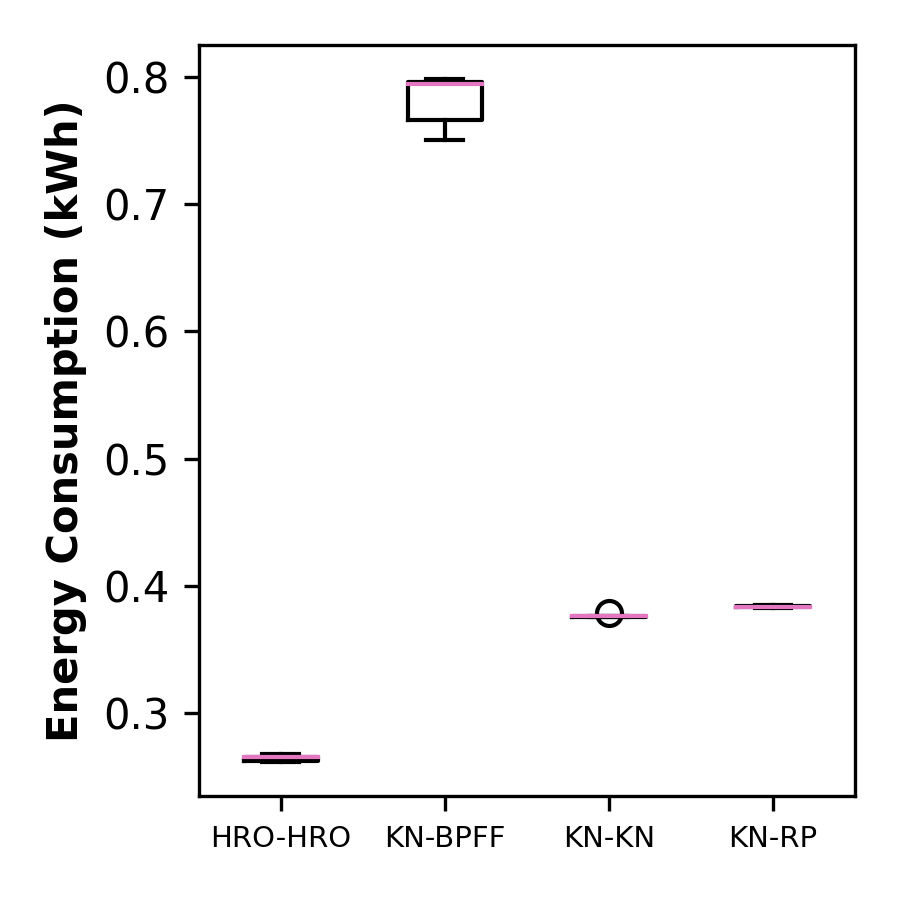
\includegraphics[width=0.28\linewidth]{4_Chapitre4/figures/evaluation/z-energy-20221212-232143-169224.png}
    }
    \caption{Evaluation 1 -- Comparison against baselines}
    \label{figure:herofake-evaluation-hro-full}
\end{figure*}

\begin{figure*}[t]
    \centering
    \subfloat[Task consolidation (based on the unused node count)\label{figure:herofake-evaluation-mixed-nodes}]{
        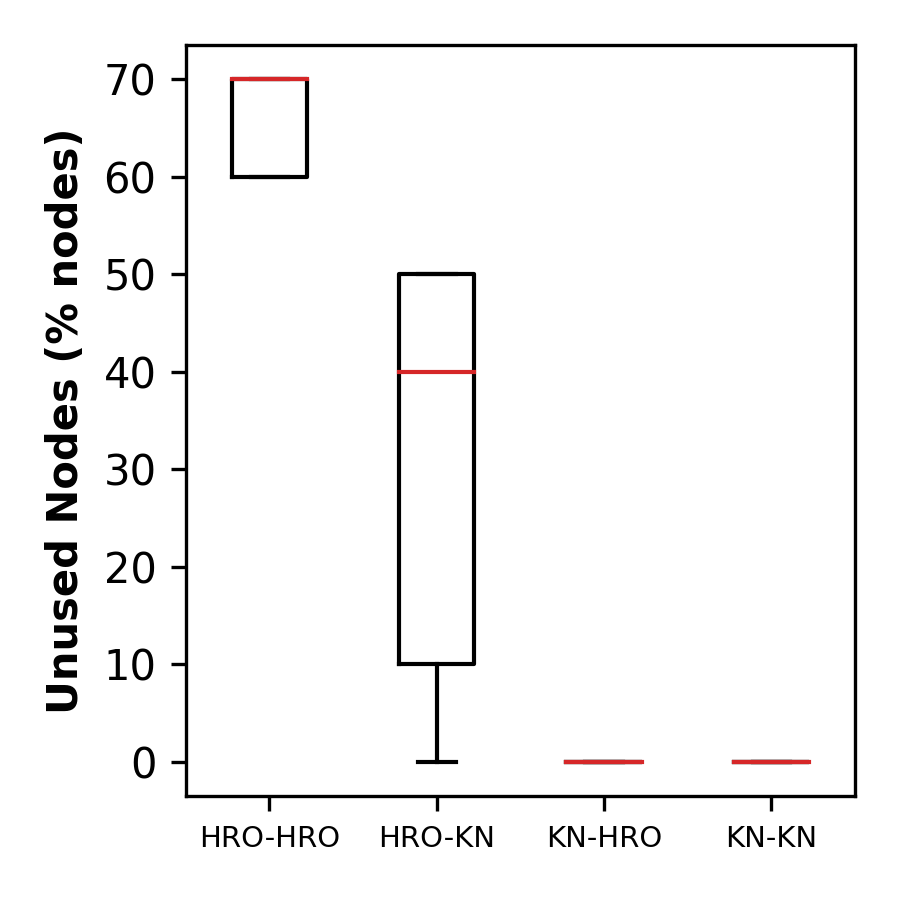
\includegraphics[width=0.28\linewidth]{4_Chapitre4/figures/evaluation/x-nodes-20221212-185844-053283.png}
    }\qquad
    \subfloat[QoS violations (based on tasks with missed deadline)\label{figure:herofake-evaluation-mixed-penalty}]{
        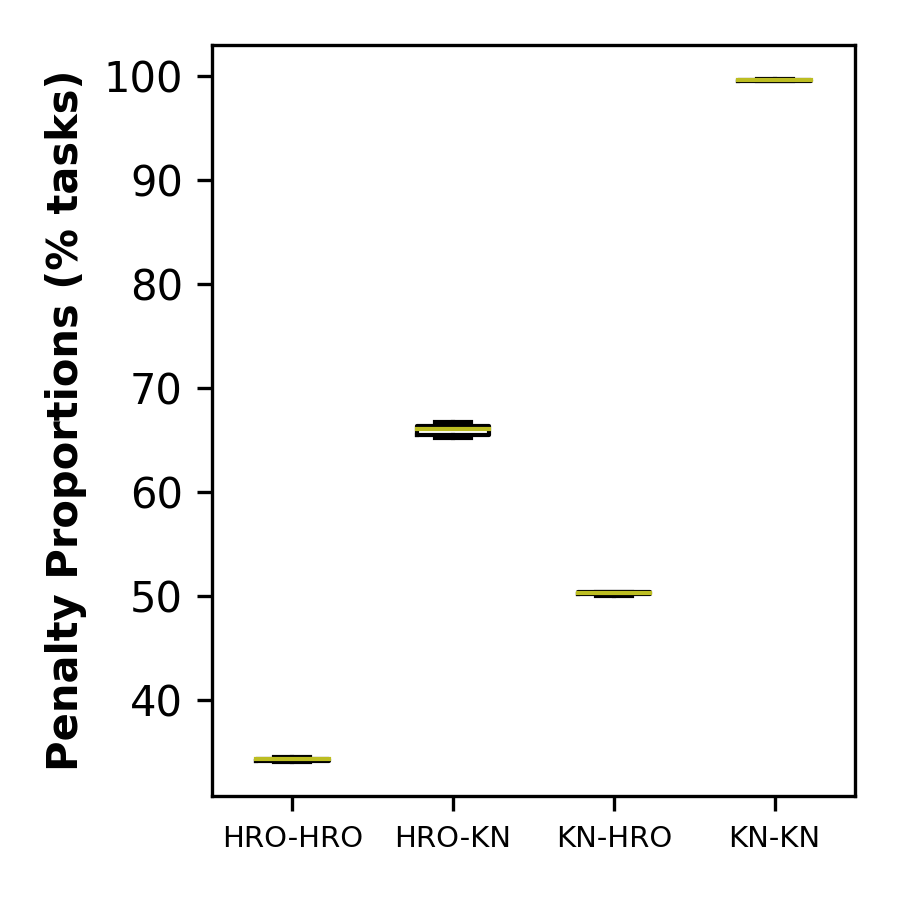
\includegraphics[width=0.28\linewidth]{4_Chapitre4/figures/evaluation/x-penalty-20221212-185844-053283.png}
    }\qquad
    \subfloat[Dynamic energy consumption (in kWh)\label{figure:herofake-evaluation-mixed-energy}]{
        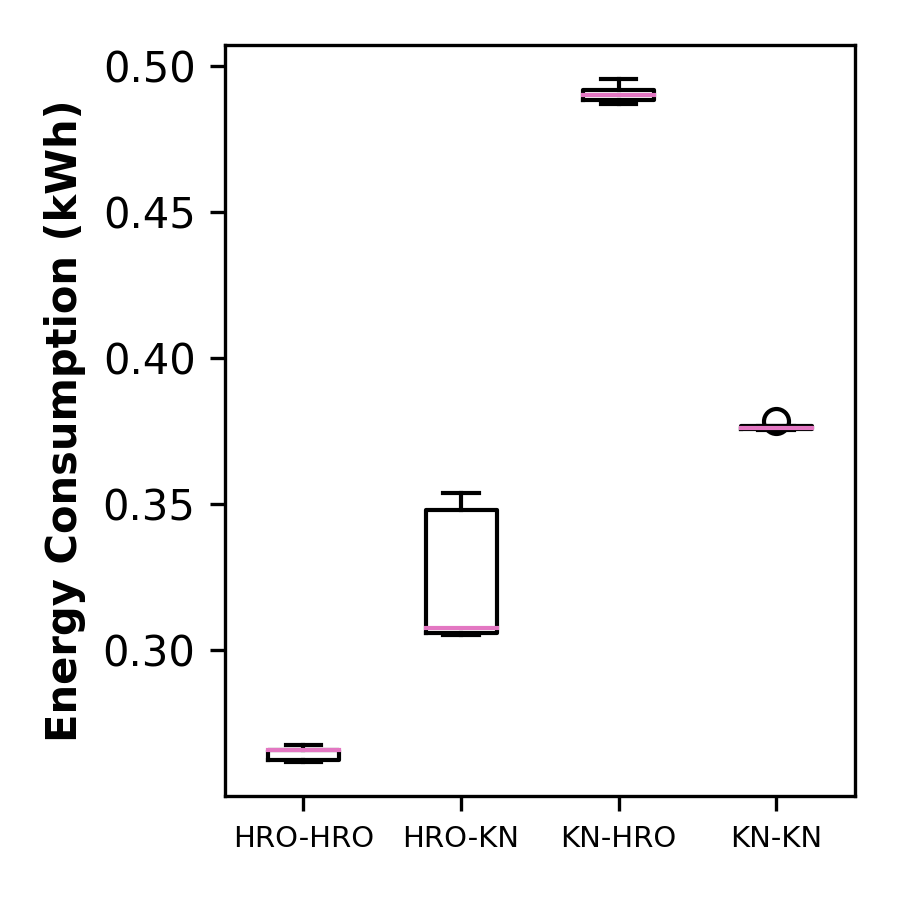
\includegraphics[width=0.28\linewidth]{4_Chapitre4/figures/evaluation/x-energy-20221212-185844-053283.png}
    }
    \caption{Evaluation 2 -- Impact of HeROfake components on the overall performance}
    \label{figure:herofake-evaluation-hro-mixed}
\end{figure*}

\subsection{Protocole expérimental}

Nous avons utilisé des mesures provenant de l'évaluation de trois modèles d'apprentissage automatique différents (voir Tableau~\ref{table:herofake-tasks}). Ces modèles ont été mis en œuvre sur trois plateformes d'exécution différentes (voir Tableau~\ref{table:herofake-platforms}) comme expliqué dans la Section~\ref{section:herofake-offline}.

Ces données ont servi d'entrée à un simulateur que nous avons construit en utilisant SimPy~\cite{simpy}. Le simulateur suit le modèle de système décrit dans les sections~\ref{model:nodes}, \ref{model:platforms}, \ref{model:tasks}.

Nous avons mesuré les délais de démarrage à froid pour les applications de notre étude de cas, voir le tableau~\ref{table:herofake-tasks}. Il apparaît que les délais d'exécution sont dominés par les délais de démarrage à froid, ce qui fait de l'allocation adéquate des ressources une exigence stricte pour respecter les accords de niveau de service.

Dans la partie consacrée à l'évaluation des performances, nous comparons deux autoscalers :

\begin{itemize}
    \item HeROfake (HRO) -- Notre allocateur de ressources basé sur les métadonnées et conscient de l'hétérogénéité ;
    \item Knative (KN) -- Nous avons modélisé le comportement de l'autoscaler Knative au mieux de nos connaissances.
\end{itemize}

Notre évaluation comporte quatre ordonnanceurs :

\begin{itemize}
    \item HeROfake (HRO) -- Notre ordonnanceur conscient des coûts qui minimise les violations de SLA, la consommation d'énergie et l'utilisation des ressources ;
    \item Knative (KN) -- Knative sélectionne une plateforme sur le nœud le plus disponible~\cite{sureshENSUREEfficientScheduling2020}. Les plates-formes d'exécution sont triées en fonction du nombre de demandes en cours d'exécution. La plateforme avec la file d'attente la plus courte est sélectionnée ;
    \item Random Placement (RP) -- Les tâches sont assignées à une plateforme d'exécution aléatoire sur un nœud aléatoire ;
    \item Bin Packing First-Fit (BPFF) -- Les tâches sont consolidées sur le nombre minimum de plateformes d'exécution. Tant qu'un nœud dispose de suffisamment de mémoire pour accueillir de nouvelles répliques, il est systématiquement choisi jusqu'à ce qu'il n'ait plus de mémoire ; un nouveau nœud est alors sélectionné. BPFF sera probablement la politique d'ordonnancement pour AWS Lambda~\cite{wangPeekingCurtainsServerlessb}.
\end{itemize}

Nous avons conçu une évaluation des performances en deux étapes basée sur des simulations :

\begin{itemize}
    \item \textbf{Comparaison avec les lignes de base} (Figure~\ref{figure:herofake-evaluation-hro-full}) : dans cette partie, nous avons comparé notre combinaison HeROfake d'autoscaler et d'ordonnanceur (HRO-HRO) à : (1) l'autoscaler et l'ordonnanceur Knative complet (KN-KN), (2) l'autoscaler Knative avec l'ordonnanceur BPFF (KN-BPFF), (3) l'autoscaler Knative avec l'ordonnanceur RP (KN-RP) ; 
    \item \textbf{Impact des composants HeROfake sur la performance globale} (Figure~\ref{figure:herofake-evaluation-hro-mixed}) : nous discutons ici de l'impact individuel de chacun des autoscalers et de l'ordonnanceur. Pour ce faire, nous avons conçu différentes stratégies : (1) en utilisant l'autoscaler HeROfake avec l'ordonnanceur Knative, et (2) en utilisant l'autoscaler Knative avec l'ordonnanceur HeROfake, et nous avons comparé ces stratégies avec les fonctionnalités complètes de HeROfake et Knative.
\end{itemize}

La dénomination de chaque scénario dans ces figures se compose de deux parties divisées par un symbole de tiret. La première partie correspond à la politique d'allocation, la seconde à la politique d'ordonnancement (par exemple, HRO-KN signifie que nous avons utilisé l'autoscaler HeROfake en conjonction avec l'ordonnanceur Knative). 

Pour chacune des combinaisons de politiques d'autoscaler et d'ordonnanceur, nous avons réalisé l'expérience sur un scénario de charge de travail synthétique composé de 50000 tâches (demandes d'utilisateurs). Les tâches se voient attribuer un type aléatoire (ResNet50, VGG16 ou VGG19) et un niveau de QoS aléatoire (élevé, moyen, faible) suivant une distribution uniforme, avec des écarts de durée de QoS respectivement fixés à 2, 3 et 4. L'infrastructure du scénario se compose de 10 nœuds (10 CPU, 6 GPU, 2 FPGA).

Les pondérations pour le niveau de concurrence (équation~\ref{eq:herofake-HRO-concurrency-target}) ont été fixées à $k_{ET} = \frac{2}{3}$, $k_{EC} = \frac{1,5}{6}$ et $k_{HP} = \frac{0,5}{6}$. Les pondérations pour la décision de réduction d'échelle (équation~\ref{eq:herofake-HRO-allocation-cost-function}) ont été fixées à $k_{TT} = \frac{2}{3}$, $k_{EC} = \frac{1,5}{6}$ et $k_{HP} = \frac{0,5}{6}$. Les pondérations pour la décision d'ordonnancement (équation~\ref{eq:herofake-HRO-scheduling-cost-function}) ont été fixées à $k_{QP} = \frac{2}{3}$, $k_{EC} = \frac{0,5}{6}$ et $k_{TC} = \frac{1,5}{6}$. 

\subsection{Analyse des résultats}

\subsubsection{Comparaison aux politiques de base}

\textbf{Consolidation des tâches}. La figure~\ref{figure:herofake-evaluation-full-nodes} montre que notre combinaison d'autoscaler et d'ordonnanceur permet d'obtenir le plus grand nombre de nœuds inutilisés. Avec l'autoscaler de Knative, l'ordonnanceur BPFF assure la meilleure consolidation, mais cette politique nécessite toujours plus de trois fois les nœuds dont nous avons besoin avec notre politique.

\textbf{Accords de niveau de service}. La figure~\ref{figure:herofake-evaluation-full-penalty} montre que HRO-HRO est le plus performant en termes de violations de la QoS, avec 35\% de tâches qui ne respectent pas les délais. Il s'agit d'une amélioration considérable par rapport aux résultats de Knative, où les tâches ne respectent pas les délais dans plus de 99\% des cas : le retard introduit par l'allocation réactive des ressources ne peut pas être compensé à temps en utilisant uniquement des unités centrales.

\textbf{Consommation d'énergie}. La figure~\ref{figure:herofake-evaluation-full-energy} montre que notre politique, avec l'autoscaler et l'ordonnanceur HRO fonctionnant conjointement, est toujours la plus performante en termes de consommation d'énergie dynamique. Cela s'explique évidemment par le fait que nous allouons des accélérateurs matériels ; cependant, au cours de notre évaluation, la durée d'exécution de notre scénario est similaire avec les politiques Knative et HRO (environ 13,5 minutes). La politique d'ordonnancement BPFF est également la moins performante en termes de temps d'exécution, car elle maximise les files d'attente des tâches dans les plateformes d'exécution, ce qui donne les pires résultats en termes de consommation d'énergie.

\subsubsection{Impact des composants individuels}

\textbf{Consolidation des tâches}. La figure~\ref{figure:herofake-evaluation-mixed-nodes} montre que HRO-HRO est le plus performant en matière de consolidation des tâches, laissant un peu moins de 70\% des nœuds disponibles inutilisés, alors que l'ordonnanceur de Knative, dans le cadre de notre politique d'autoscaling, n'atteint que 40\% de nœuds inutilisés. Ce résultat est attendu, car l'ordonnanceur de Knative utilise une politique de moindre connexion. Les résultats de consolidation de KN-HRO sont médiocres, mais pour une raison différente : notre ordonnanceur tente de minimiser les violations de la qualité de service et répartit la tâche sur tous les processeurs alloués.

\textbf{Accords de niveau de service}. La figure~\ref{figure:herofake-evaluation-mixed-penalty} montre que notre ordonnanceur ne fonctionne pas bien en conjonction avec l'autoscaler de Knative. En effet, notre ordonnanceur tente de minimiser les pénalités : lorsqu'il ne dispose que de CPU, il se comporte de la même manière que l'ordonnanceur de Knative et répartit les tâches sur ces CPU afin de limiter les violations de la qualité de service. Cependant, notre ordonnanceur sous l'autoscaler Knative parvient toujours à maintenir les violations de la qualité de service à environ 50\% des tâches, ce qui montre qu'il y a une marge d'amélioration même lorsque les tâches d'inférence sont déployées sur des CPU uniquement. Notez que lors de notre évaluation, l'autoscaler Knative a donné les pires résultats en ce qui concerne la fréquence des démarrages à froid (6,5 fois plus fréquents avec KN-HRO qu'avec HRO-KN).

\textbf{Consommation d'énergie}. La figure~\ref{figure:herofake-evaluation-mixed-energy} montre que la consommation d'énergie est toujours plus faible lorsque l'on utilise notre autoscaler, qui peut allouer des accélérateurs matériels. Cependant, notre planificateur utilisé avec l'autoscaler de Knative donne les pires résultats en termes de consommation d'énergie. Cela s'explique à nouveau par le fait que l'ordonnanceur tente de minimiser les pénalités et de répartir les tâches sur un nombre maximal de CPU.

\section{État de l'art}
\label{section:herofake-sota}

Les travaux antérieurs se sont concentrés sur les plates-formes de mise à l'échelle automatique pour le déploiement de tâches de courte durée, comprises dans des applications présentant des modèles de charge imprévisibles. Le tableau~\ref{table:herofake-sota} résume les différences entre ces contributions et notre plateforme cible.

Certaines de ces contributions ont tenté d'atteindre le SLA avec des ressources non réservées~\cite{gujaratiSwayamDistributedAutoscaling2017, zhangMArkExploitingCloud, mampageDeadlineawareDynamicResource2021, singhviAtollScalableLowLatency2021, handaoui2020releaser, handaoui2020salamander, yalles2022riscless}.
Parmi ces contributions, certaines se concentrent sur l'utilisation de ressources matérielles hétérogènes supplémentaires pour accélérer l'exécution de la charge de travail~\cite{zhangMArkExploitingCloud, lingPigeonDynamicEfficient2019, yangINFlessNativeServerless2022}.
Elles nécessitent souvent un surprovisionnement des ressources pour utiliser l'accélération matérielle, par exemple en s'appuyant sur des instances AWS réservées qui donnent accès aux GPU~\cite{zhangMArkExploitingCloud}, en utilisant un pool de conteneurs préchauffés~\cite{lingPigeonDynamicEfficient2019}, ou même en provisionnant de manière proactive les nœuds pour respecter les délais des fonctions définies par l'utilisateur~\cite{singhviAtollScalableLowLatency2021}. Ces solutions intéressantes peuvent toutefois s'avérer insuffisantes en termes d'utilisation des ressources et entraîneraient une consommation d'énergie supplémentaire dans un cloud privé.

En outre, certains auteurs se concentrent sur des infrastructures homogènes \cite{gujaratiSwayamDistributedAutoscaling2017, sureshENSUREEfficientScheduling2020, mampageDeadlineawareDynamicResource2021, singhviAtollScalableLowLatency2021, yangINFlessNativeServerless2022}. Ces études pourraient difficilement s'adapter au contexte du cloud privé que nous visons, où les ressources sont généralement transitoires et hétérogènes. En outre, certaines de ces contributions proposent des modèles de tâches qui ne couvrent pas les accords de niveau de service définis par l'utilisateur et par demande~\cite{sureshENSUREEfficientScheduling2020, lingPigeonDynamicEfficient2019}. Enfin, certaines de ces contributions sont axées sur les performances plutôt que sur les coûts, ce qui est crucial dans notre contexte de cloud privé~\cite{gujaratiSwayamDistributedAutoscaling2017, lingPigeonDynamicEfficient2019, singhviAtollScalableLowLatency2021, choSLADrivenMLInference}.

Bien que l'alimentation soit l'un des éléments les plus importants du coût total de possession (TCO) dans un centre de données - dépassant parfois le coût d'achat du matériel~\cite{7279063} -- à notre connaissance, aucune de ces contributions ne couvre l'impact de l'allocation et du placement dynamiques sur la consommation d'énergie, ni ne considère la consommation d'énergie comme une mesure de la qualité de service. Il s'agit d'une limitation sérieuse, car l'optimisation de la consolidation des tâches ouvre la voie à des politiques d'étranglement et de mise hors tension qui peuvent avoir un impact majeur sur l'efficacité énergétique d'un centre de données~\cite{chaurasiaComprehensiveSurveyEnergyaware2021}.

\section{Conclusion et perspectives}

Dans cet article, nous avons présenté HeROfake, notre cadre pour le déploiement de tâches de détection de deepfake interactives et de courte durée sur un cloud privé hétérogène serverless.

Nous avons présenté les deux phases qui composent ce cadre : une phase hors-ligne au cours de laquelle nous caractérisons les performances des plateformes d'exécution et les exigences des tâches ; et une phase en ligne au cours de laquelle nous allouons dynamiquement les ressources et planifions les tâches à exécuter sur ces plateformes.

Les résultats expérimentaux montrent que si le temps total d'exécution des tâches dans HeROfake est similaire à celui de la version vanille de Knative, nous obtenons une réduction de plus de 60\% des pénalités de qualité de service ; les tâches sont consolidées sur moins de 40\% des nœuds de l'infrastructure, 77\% des plates-formes d'exécution restant inutilisées ; enfin, la consommation d'énergie dynamique est réduite de 35\% par rapport à Knative.

L'inclusion du traitement vidéo dans le cadre est un défi intéressant, car il introduirait des dépendances entre les tâches. Les exécutions de fonctions ne seraient plus \textit{stateless}, ce qui entraînerait la nécessité de s'attaquer au problème du stockage des données intermédiaires dans une infrastructure serverless.

Nous avons également l'intention d'étendre le simulateur avec un analyseur syntaxique afin d'être en mesure d'utiliser des traces de centres de données réels comme scénarios d'entrée, au lieu d'utiliser uniquement des charges de travail synthétiques.
